\documentclass[11pt]{article}

\usepackage{amsmath,amssymb}
\usepackage{a4wide}
\usepackage{graphicx}
\usepackage{tikz}
\usepackage{algorithm}
\usepackage{algorithmic}
\usepackage{parskip}
\usepackage{caption}
\usepackage{subcaption}
\usepackage{gensymb}

\newcommand{\maxsize}[1]{\begin{quotation} {\sl \noindent Maximum size: #1.} \end{quotation}}

\newcommand{\crp}[1]{\begin{quotation} {\sl \noindent For the curve- and network-reconstruction problem: #1} \end{quotation}}

\newcommand{\example}[1]{\begin{quotation} {\sl \noindent Example: #1} \end{quotation}}

%%
% Theorem-Like Environments
%
\newtheorem{defin}{Definition}
  \newenvironment{mydefinition}{\begin{defin} \sl}{\end{defin}}
\newtheorem{theo}[defin]{Theorem}
  \newenvironment{mytheorem}{\begin{theo} \sl}{\end{theo}}
\newtheorem{lem}[defin]{Lemma}
  \newenvironment{lemma}{\begin{lem} \sl}{\end{lem}}
\newtheorem{coro}[defin]{Corollary}
  \newenvironment{corollary}{\begin{coro} \sl}{\end{coro}}
\newtheorem{obse}[defin]{Observation}
  \newenvironment{observation}{\begin{obse} \sl}{\end{obse}}

\newenvironment{proof}{\emph{Proof.}}{\hfill $\Box$ \medskip\\}

% TODO(robwu): Choose a more descriptive title
\title{2D curve and network reconstruction}
\author{
A. van den Boogaart \and
W. Brouwer \and
C. Mens \and
M. Muijsers \and
R. Wu
}
\date{\today}

\begin{document}

\newpage

\maketitle

\begin{abstract}
In this study  two formulations of solutions to effectively solve the problem of connecting a set of nodes in the 2D plane in an aesthetically pleasing manner, and one formulation of a solution for reconstructing a road network from a set of nodes in the 2D plane are proposed.
The first proposed solution reconstructs these nodes into a single curve.
The second proposed solution will yield a similar result as the first solution, but will distinguish multiple curves from one another.
The third proposed solution attempts to create a road network from nodes. This problem is distinct from the other two, as here the challenge lies in creating intersections, instead of avoiding them.

\end{abstract}

\section{Introduction}
\label{se:introduction}
The to be presented algorithms will solve the problem of reconstructing curves for a given set of points in the 2D plane. This problem has three slightly different forms: The first two require the reconstruction of a set of points into curves, in the first case there is only one curve, whereas in the second case there are multiple. The third part of the problem requires reconstructing to a road network.

To be able to focus on a specific type of curve reconstruction, we will only consider curves where all points in the input are used and where line segments do not intersect each other.

The goal of the road network algorithm is to create a reasonable representation of the road network, such that a person would agree with the representation that the algorithm gives. This algorithm could be used to create a road map from the given data.

As with the other two algorithms, we have created some constraints for the road network to be able to focus on specific input. All points need to have at least one possible path to every other point and intersecting lines need an additional node at the intersection. The nodes are points in a 2D plane. In practice, the generation of nodes can be done by laser scanners, or in the case of the road network, by following roads and giving a gps location at certain intervals.

There are multiple known solutions to these problems. One of these is `The Crust Algorithm' \cite{crust}, which first creates a Voronoi diagram, then uses Delaunay triangulation between the Voronoi diagram and the Voronoi vertices. The Crust Algorithm works well in three dimensions, but has difficulty with detecting sharp corners which are common in two dimensional reconstruction.
A different algorithm, specifically made for two dimensional reconstruction is `Gathan' \cite{gathan}. This provides a good solution for general cases, but does not allow for selecting multiple or single curves and relies on difficult mathematical graphs.
DISCUR \cite{discur} is another algorithm solving the curve reconstruction problem. It has no parameters, but requires dense sampling points to recontruct correctly.
For the network problem there exists a road network reconstruction algorithm \cite{chen} which obtains subcurves by creating a voronoi diagram.

Delaunay triangulation could possibly be used to create a relatively small set of edges for the third problem, after which a rectilinear spanning graph or straight lines can be determined between points. This will improve efficiency, as it has a running time of $O(n \log{n})$, whereas Kruskal's algorithm will check all possible edges initially, resulting in $O(n^2 \log{n})$.

For the single curve reconstruction problem, we have also looked at the convex hull \cite{convex}. A convex hull will create segments between all the outermost points, such that no unconnected point is outside of the enclosed area. Like putting a rubber band around all the points. This is useful for the outermost nodes, but does not do anything with the nodes inside this outline.

For solving these three problems, we present an algorithm for each problem.
To solve the single curve reconstruction problem, the algorithm creates a convex hull and then continues by removing the largest edge and then reconnecting the figure by creating 2 new segments with another nearby point.
Multiple curves are solved using a seperate algorithm, which first connects the shortest segments such that there are no intersecting lines, after which it will seek out sharp angles and tries to remove and replace these with obtuse angles.
The road network reconstruction problems is solved using a minimum spanning tree. After reconstructing this tree, the algorithm finds nodes with degree 1 and connects these to a nearby node. To correctly create intersections, nodes with degree 3 or higher will check their surrounding segments and will add a point based on their angles.

\begin{figure}[ht!]
\centering
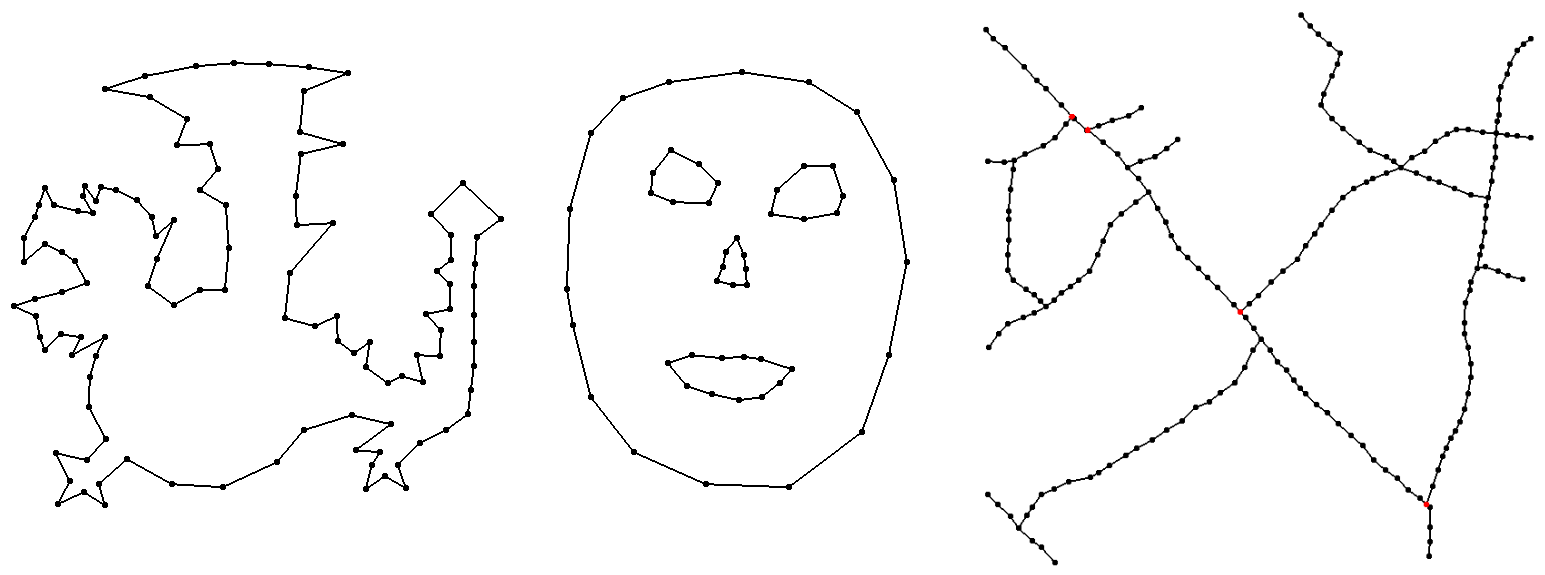
\includegraphics[scale=0.3]{images/outputOverview.png}
\caption{Output of the single curve (Left), multiple curve (Middle) and Network (Right) reconstruction algorithms.}
\label{outputOverview}
\end{figure}$ $\\


\section{The algorithms}
\label{se:algorithms}
\subsubsection{Background definitions}
Let $U = [0,1]^2$ be a set of points in a two-dimensional space.
For any $u,v \in U$, the line segment between $u$ and $v$ is denoted as $s_{u,v}$. $u$ and $v$ are called the endpoints of $s_{u,v}$. Each of the presented algorithms take $P \subset U$ as input, and output $S \subset \{s_{p,q} | p,q \in P \land p \neq q \}$.
 Two distinct points $a$ and $b$ are called \textit{connected} if there is a segment in $S$ whose endpoints are $a$ and $b$.
 Two segments are \textit{intersecting} each other if the line segments have a common point besides than the endpoints.
%TODO (rob): The next line does not belong here, it's a detail specific to the algorithm, right?
%None of these output line segments intersect another line segment in $S$.

For any $p,q \in U$, $d(p,q)$ is the Euclidean distance between $p$ and $q$. %\ref{todo:euclid_distance}.

For every $p \in P$ and $n \in \mathbb{N}$, $Adj_{p,n}$ is an adjacency list consisting of the $n$ nearest points to $p$, sorted in ascending order.

For any $p \in P$, the degree of $p$ denoted by $deg(p)$ is the number of line segments that are connected to $p$.

$\varphi(s_{u,v}, s_{v_w})$ is the absolute value of the smallest angle between two segments that share a common point,
If $p \in P$ has degree two, then $\alpha_p$ is defined to be the absolute value of the smallest angle between its two connected segments. %TODO What if degree is not two?



\subsection{Single curve reconstruction}
\subsubsection{Description}
For a given set of $n$ points $P \subset U$, this algorithm will generate a set of non-intersecting line segments $S$ such that:

\noindent\begin{enumerate}\topsep=0pt\itemsep=0pt\parsep=0pt
\item $\forall p \in P : deg(p) \leq 2$
\item The segments in $S$ do not intersects each other
\end{enumerate}

Furthermore, the algorithm will in many practical cases conform to the following requirement:

\noindent\begin{enumerate}\topsep=0pt\itemsep=0pt\parsep=0pt
\item The segments form an open or closed curve, i.e. $\#S = n-1 \vee \#S = n$
\end{enumerate}

The algorithm is based on the idea that a single curve always can be outlined by some concave polygon, and therefore we start with an outline of the points, after which we collapse this outline into the remaining points inside this polygon.

Collapsing an outline such that the resulting polygon will contain all points implies all points must be inside the polygon defined by this outline. For this purpose, we start with generating the convex hull as our initial set of segments. To compute the convex hull, we will use the Graham scan\cite{convex}, an algorithm that finds all vertices of the convex hull ordered along its boundary.

The algorithm thus begins by creating a set $S$ of segments that make up the convex hull of $P$. After that we define a likelihood function, for which two existing possibilities are listed below:

\noindent\begin{enumerate}\topsep=0pt\itemsep=0pt\parsep=0pt
\item $s_{u,v} \in S \wedge p \in P \Rightarrow likelihood(s_{u,v}, p) = d(u, v)*d(u, v)/(d(p, v)*d(p, v)+d(p, u)*d(p, u))$
\item $s_{u,v} \in S \wedge p \in P \Rightarrow likelihood(s_{u,v}, p) = d(u, v)/d(p, v)+d(p, u))$
\end{enumerate}

Then, let $Q = \{ p \in P | \neg ( \exists v \in P \exists s_{p,v} \}$. Then $\#Q = n - \#S$.

After the convex hull boundary vertices are found, we will start repeating the following procedures until $\#Q = 0$:

\begin{enumerate}
\item Let $p \in P$ be a point and $s_{u,v} \in S$ be a segment so that $q \in P \wedge t \in S \Rightarrow likelihood(s_{u,v}, p) \geq likelihood(t, q)$
\item Remove $s_{u,v}$ from $S$
\item Add $s_{u, p}$ to $S$
\item Add $s_{v, p}$ to $S$
\item Remove $p$ from $Q$
\end{enumerate}

This way, we get a curve defined by the segments in $S$ with exactly as many segments as given in the input. Since for every point in $Q$, we add one segment in $S$, resulting in $\#S = n$.

These operations can however give intersecting segments, and also segments that are extremely long and are likley not part of the correct solution. To solve these issues, the algorithm will remove all lines that seem inappropriate.

Let $l1(S)$ be the longest segment such that $l1(S) \in S$, and let $l2(S)$ be the longest segment so that $l2(S) \in S \setminus { l1(S) }$. Then to remove all segments that could be too long we compare the factor between the two longest segments to some parameter $k$:

\begin{enumerate}
\item While $l1(S) \geq k \cdot l2(S)$, remove $l1(S)$ from $S$
\end{enumerate}

Then, the algorithm will remove any intersections that are left, by starting with removing the segments that have the largest amount of intersections:

\begin{enumerate}
\item Let $s \in S \Rightarrow I(s) = \{ t \in S | s$ intersects with $t \}$. Then, until $s \in S \Rightarrow \#I(s) = 0$, remove $r$ from $S$, where $s \in S \Rightarrow \#I(s) \leq \#I(r)$
\end{enumerate}

This can greatly reduce the size of $S$, which would invalidate the requirement of $\#S=n$. If there are segments $s_{u,v}$ such that $deg(u) = 1$, $deg(v) = 1$, $\neg ( s_{u,v} \in S )$ then $s_{u,v}$ could be a good candidate to add to $S$. The algorithm will, in an attempt to repopulate $S$, add any such segments $s_{u,v} \in MST(P) $, where $MST(P)$ denotes the set of segments representing a minimum spanning tree of $P$. Again, a very long segment may have been re-added. To prevent this from showing up in the final result, the algorithm tries to remove a segment that is too long one more time:

\begin{enumerate}
\item If $l1(S) \geq k \cdot l2(S)$, remove $l1(S)$ from $S$
\end{enumerate}

A basic implementation of the algorithm requires $O(n^2)$ time, assuming a running time of a Graham scan implementation of $O(n\log(n))$ and a running time of a minimum spanning tree implementation of $O(n\log(n))$. It may run using $O(n^2)$ or $O(n)$ storage, depending on how the likelihoods are compared. If memory is slow, an index of likelihoods from every segment in $S$ to every point in $Q$ can be kept and updated, resulting in $O(n^2)$ storage. Otherwise, these likelihoods can be recalculated when needed, resulting in $O(n)$ storage.

\subsection{Multiple curve reconstruction}
\subsubsection{Description}
For a given set of $n$ points $P \subset U$, this algorithm generates a set of non-intersecting line segments $S$ such that for every point, its degree is at most two.
The segments in $S$ connect points in $P$ and form one or more shapes.
$S$ is generated in two steps. At first, $S$ is filled with segments by a distance-based algorithm. Then, segments in this set are replaced using an algorithm that also accounts for angles.

During both steps, two invariants are maintained:%
\noindent\begin{enumerate}\topsep=0pt\itemsep=0pt\parsep=0pt
\item $\forall p \in P : deg(p) \leq 2$
\item The segments in $S$ do not intersect each other.
\end{enumerate}

%First, a set of segments is generated from the input. From this set, the shortest segments are selected and added to $S$ if the invariants are not invalidated. More precisely:

%TODO Arjan said that it would be a good idea to first explain how T is generated before stating how it is used.
Let $T \subset \{s_{p,q} | p,q \in P \land p \neq q \}$. A segment $s_{shortest}$ is said to be the shortest segment if there is no other segment in $T$ whose length is smaller than the length of $s_{shortest}$.
While $T$ is not empty, find $s_{shortest}$, remove it from $T$ and add it to $S$ if doing so does not invalidate the invariants. Repeat this step until $T$ is empty.
%TODO Early termination is also possible when $S$ has $n$ elements.

%TODO Justify previous method.

The elements for set $T$ can be generated in two ways. A straight-forward approach is to create a list of all possible segments, sort the list by segment lengths and iterate over the list. The number of possible segments is $(n-1)^2$, so the memory complexity is $O(n^2)$. Sorting time is linearithmic in terms of the number of elements to sort, so the time complexity is $O(n^2\log(n))$.

A quadratic complexity for memory is highly undesirable, because most computer systems have a limited amount of memory. To reduce the memory requirements, the first step can also be calculated using the following alternative method. For each point $p \in P$, find the $m$ nearest points and store the segments that are constructed from these points in a list. Then as before sort the list and iterate through its elements.

With this alternative method, the memory complexity is reduced to $O(mn)$. The $m$ nearest points can be found in $O(mn)$ time with partial selection sort.
%TODO Add reference for partial selection sort.
 $mn$ segments will thus be generated in $O(mn^2)$ time and sorted in $O(mn\log(mn))$ time. If $m$ is a (small) constant, then the memory complexity is $O(n)$ and the time complexity is $O(n\log(n))$. This is a huge improvement over the previous algorithm! The disadvantage of this method over the previous is that a dense cluster of $m$ points will never be connected to other points and leave gaps in a curve.

This first step only accounts for the lengths of the segments, not for any other properties of the shapes in the graph, such as the angle between two segments. $S$ could therefore contain segments that form a small angle with other segments.
A point in a bend of a sparse curve is occasionally slightly closer to another point in the same bend than any other point. Consequently, the initial set of segments form a collection of small curves that are not interconnected, as seen in figure \ref{fig:multiple_initial_solution}. Since these small curves are often triangles, it will be referred to as the "triangle problem" from now on.

\begin{figure}[hbtp]
\centering
\begin{subfigure}{.33\linewidth}
  \centering
  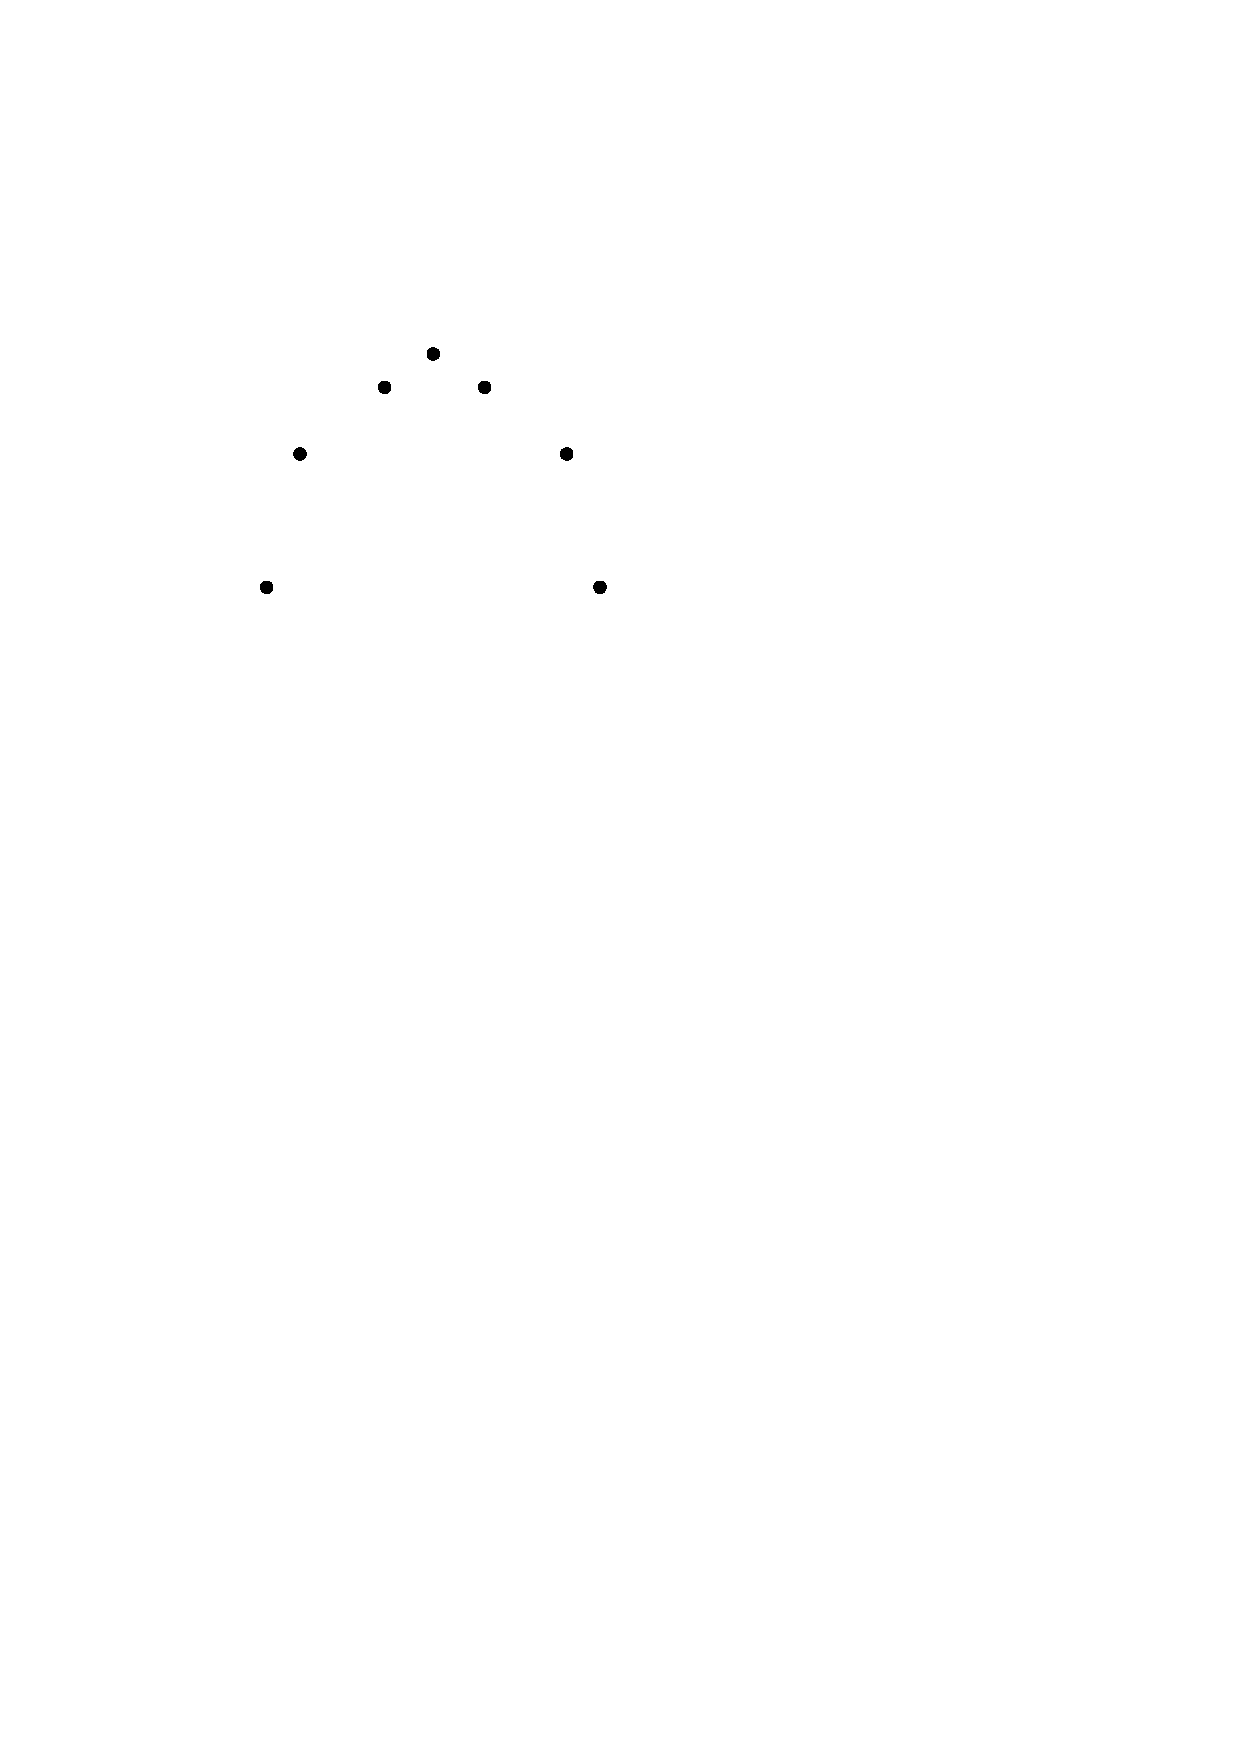
\includegraphics[width=0.9\linewidth]{multiplecurves/algo_step0_dots.pdf}
  \caption{Input}
\end{subfigure}%
\begin{subfigure}{.33\linewidth}
  \centering
  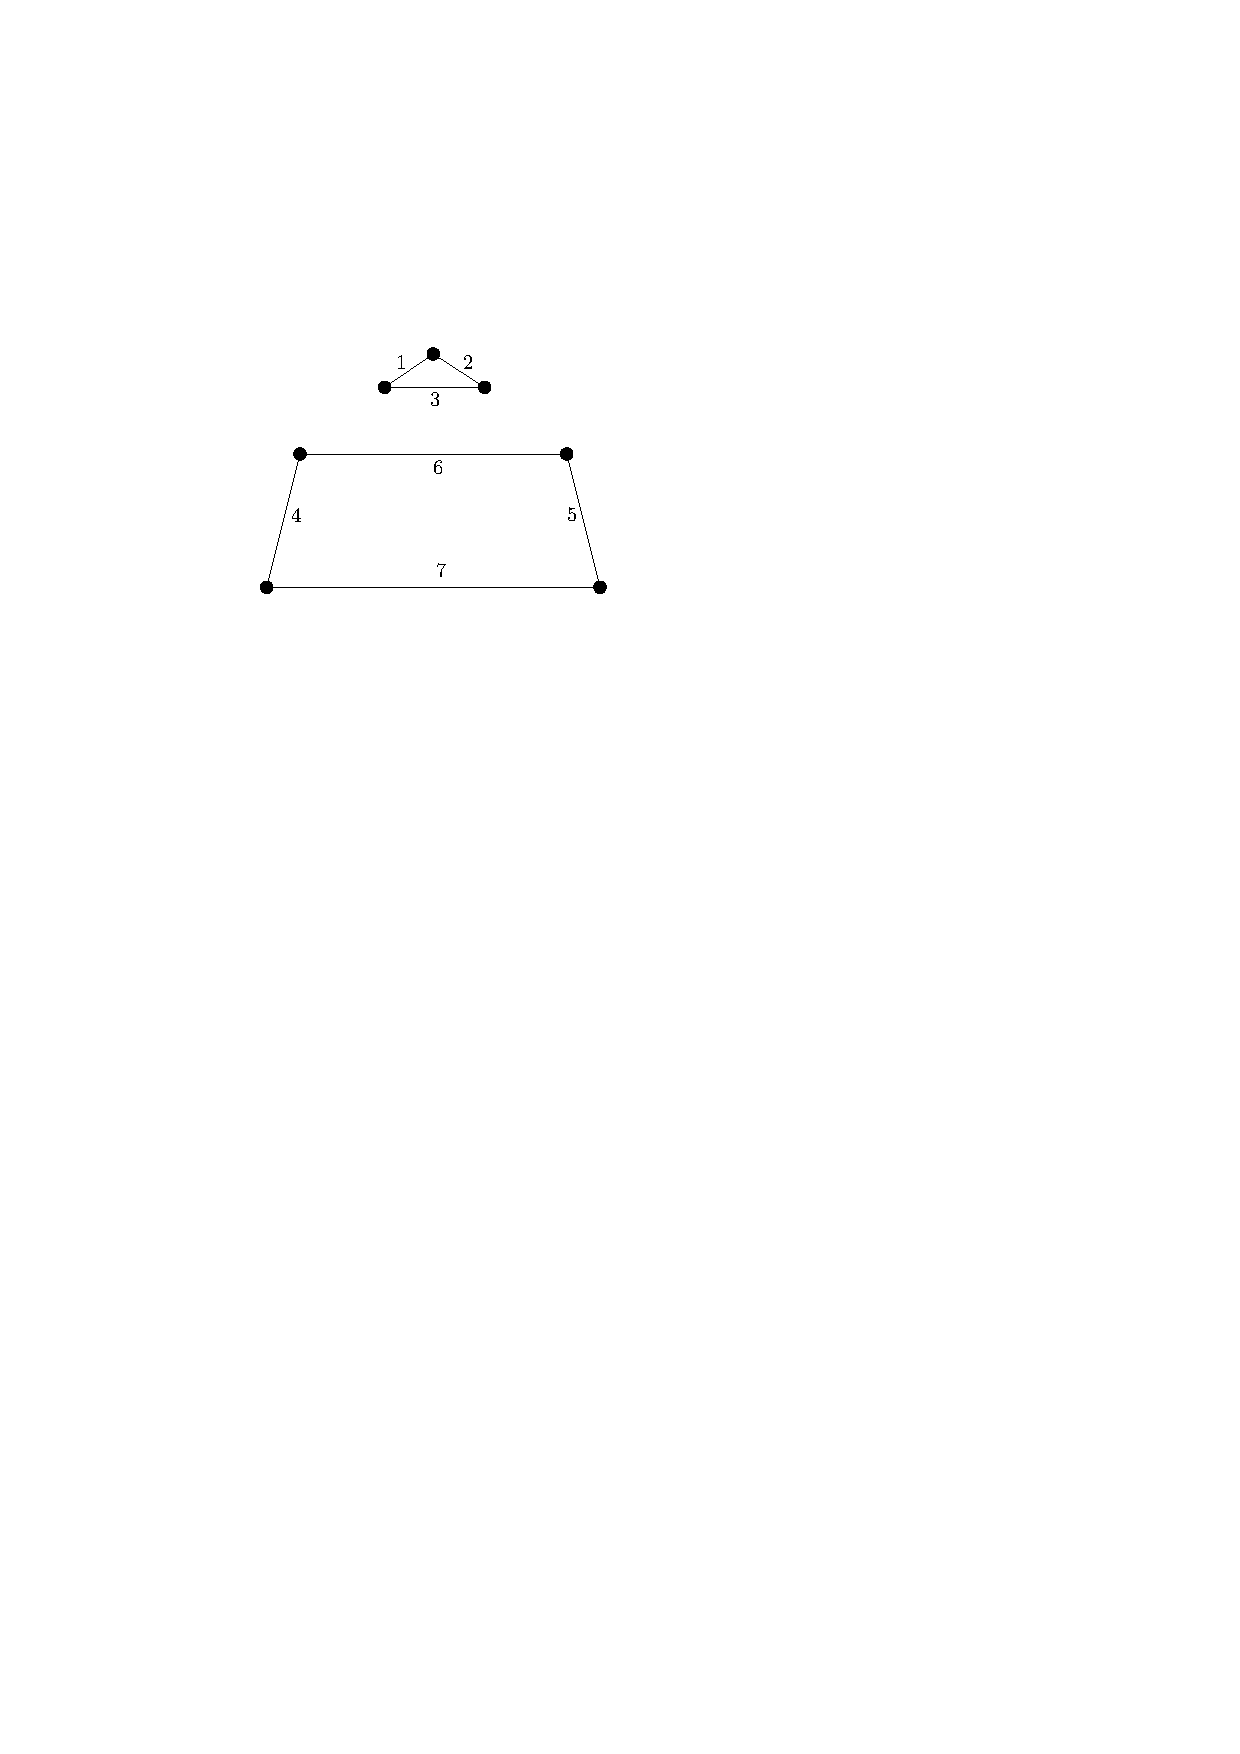
\includegraphics[width=0.9\linewidth]{multiplecurves/algo_step1_add_lines_with_numbers.pdf}
  \caption{Initial solution}
\end{subfigure}%
  \caption{Input and output of the multiple curve algorithm's first step.}
\label{fig:multiple_initial_solution}
\end{figure}

After generating the initial set of segments, disconnected shapes are joined by replacing segments in $S$ that are part of a corner with a sharp angle, if possible. Since the previous step yields a good initial solution, most of the segments will not be modified, so the angles at the endpoints of most segments will not change. This observation is important, because replacing a segment affects the angles of the segments that are connected to the former and new endpoints of the replaced segment, which could invalidate previous calculations that relied on the angles.

For every $p \in P$ where $deg(p) = 2$, select $p$ for the next step of the algorithm if $\alpha_p < \alpha_{required}$. $\alpha_{required}$ is a parameter that is used to determine whether an angle is considered to be too sharp. It is set to $90\degree$.

For each of the selected points, try to replace a segment as follows:

\begin{enumerate}
\item Let $p_1$ be the selected point, and $s_{p_1,p_2}$ be the longest segments that is connected to $p_1$. The other segment is connected to $p_3$.
\item Now try to find the best point among $Adj_{p_1,10}$. The best point is a point with degree 1 or 2 that has the optimal weight according to the following steps. The point is always accompanied by a neighbor point that is used in step \ref{multi-algo-replace}.
For every point $q_1 \in Adj_{p_1,10}$, determine the points that are connected to it. For each combination of $q_1$ and $q_2$, follow the following steps:
  \begin{enumerate}
  \item If $\varphi(s_{p_1,p_3}, s_{p_1,q_1}) < \alpha_{sharp}$, then $q_1$ is not the best point. $\alpha_{sharp}$ is a parameter that specifies the minimum required angle. This step exists to prevent inserting sharp corners again. This parameter is typically lower than $\alpha_{required}$ and is set to $45\degree$.
  \item If $d(p_1, q_1)$ and $d(p_2,q_2)$ are both greater than $d(p_1,p_3) \cdot \textsc{DistanceMultiplier}$, then $q_1$ is not the best point.
  This step ensures that a segment is not replaced by segments that are significantly shorter.
  Parameter $\textsc{DistanceMultiplier}$ is set to $1.2$ to allow points that result in a slightly shorter segment to be considered as best point.
  \item If $s_{q_1,q_2}$ is already in $S$, and (indirectly) connected to $p_1$, then $q_1$ is not the best point. This step exists to avoid breaking shapes in even smaller shapes. Since the degree of every point is at most two, this can easily be checked by enumerating the segments in the paths originating from $p_1$.
  \item If any of the new segments is close to the endpoints of the other new segment, then $q_1$ is not the best endpoint. A point is close to a line segment if the length of the line segment is greater than the distance between the point and the segment multiplied by parameter $\textsc{ClosenessFactor}$ (set to $5$).
  \item If any of the new segments intersect each other or other segments in $S$ (besides the to-be-removed ones), then $q_1$ is not the best point.
  \item Otherwise, $q_1$ is the best point if $d(p_1,q_1) + d(p_2,q_2) - d(p_1,p_2) - d(q_1,q_2)$ is minimal (relative to all other $q \in Adj_{p_1,10}$), \textit{and} greater than $\textsc{minWeight}$. This parameter specifies the threshold for the weight. A positive value means that the sum of the new segment's lengths must be smaller than the existing segments, while a negative value means that the sum is allowed to be bigger. If its value is too high, then segments will never be reconnected. When the threshold is too low, then segments are replaced regardless of the suitability of the new segments. $\textsc{minWeight}$ is set to $-0.2$.
  \end{enumerate}

\item\label{multi-algo-replace} If the best point $q_1$ exists, remove $s_{p_1,p_2}$ and $s_{q_1,q_2}$ from $S$, and add $s_{p_1,q_1}$ and $s_{p_2,q_2}$ to $S$.
If $deg(q_1) = deg(q_2) = 1$, put $s_{q_1,q_2}$ back in $S$.
\item Otherwise the longest segment cannot be replaced, so check whether the shortest segment can be replaced by repeating these steps with the shortest segment instead of the longest one.
\end{enumerate}


The meaning and relations between $p_1$, $p_2$, $p_3$, $q_1$ and $q_2$ are displayed in figure \ref{fig:multiple_pppqq}.
Let $n$ be the size of $P$. Since $|S| \leq |P|$, $|S| = O(n)$.
In the worst case, the algorithm checks for each segment whether it needs to be replaced.
During each check, the best point is selected among the 10 nearest points (found in linear time using partial selection sort).
Finding the best point takes $O(n)$ time, because a point is either eliminated in one of the constant-time checks and weight calculation, or approved after verifying in $O(n)$ time that it does not intersect the other segments.
Thus the time complexity is $O(n^2) = O(n^2)$. The storage complexity is constant.

If the first method of step 1 is used, then the full algorithm requires $O(n^2)$ storage and $O(n^2\log(n))$ time. If the alternative method is used, then the algorithm runs in $O(n^2)$ time using $O(n)$ storage.

\begin{figure}[hbtp]
\centering
\begin{subfigure}{.33\linewidth}
  \centering
  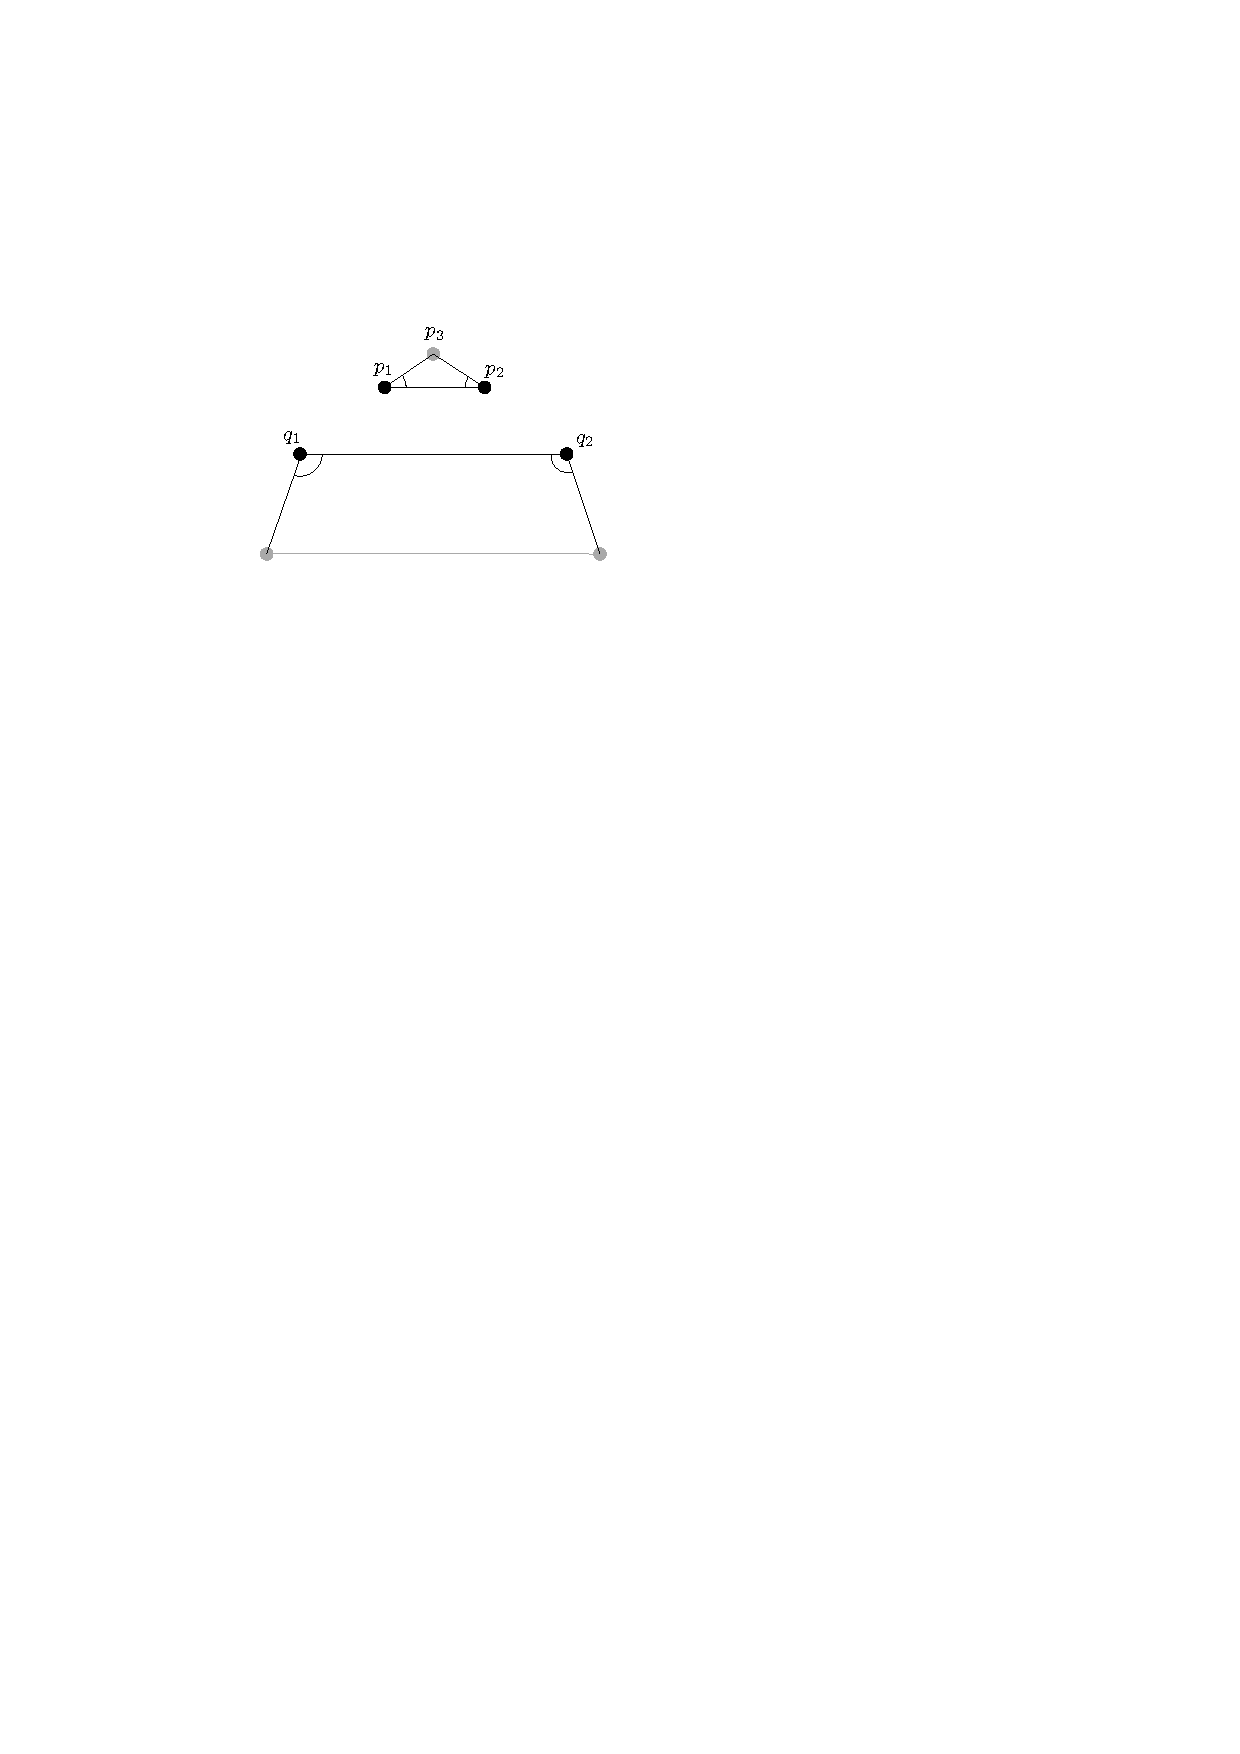
\includegraphics[width=0.9\linewidth]{multiplecurves/algo_replace_segment.pdf}
  \caption{Initial solution}
\end{subfigure}%
\begin{subfigure}{.33\linewidth}
  \centering
  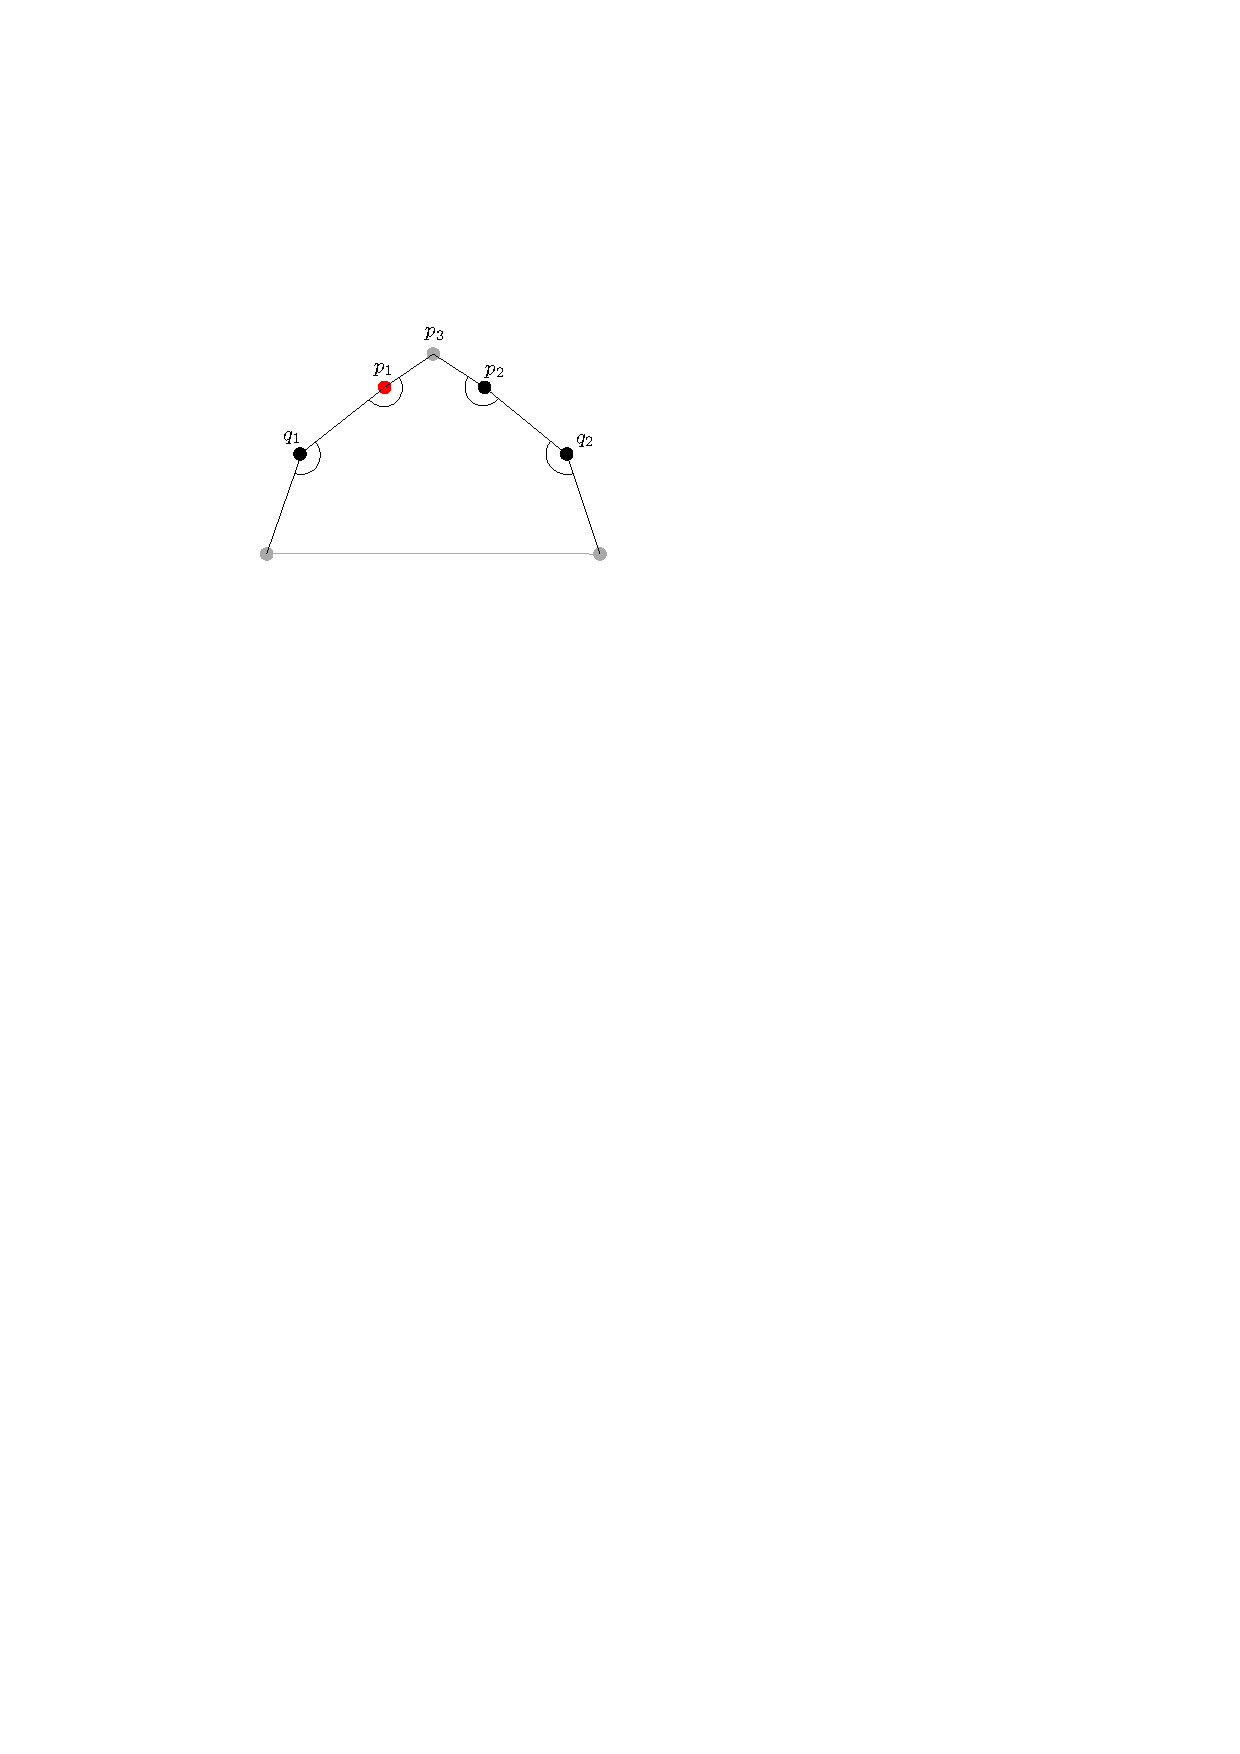
\includegraphics[width=0.9\linewidth]{multiplecurves/algo_final.pdf}
  \caption{Final solution}
\end{subfigure}%
  \caption{$s_{p_1,p_2}$ and $s_{q_1,q_2}$ is replaced with $s_{p_1,q_1}$ and $s_{p_2,q_2}$.}
\label{fig:multiple_pppqq}
\end{figure}


\subsection{Network Algorithm}
\subsubsection{Outline}
The algorithm consists of the following steps:
\begin{enumerate}
  \item Compute the $EMST$ of $P$.
  \item Find points with degree 1 and connect, if possible, to a nearby node.
  \item Find segment that divert from straight roads and remove these segments from the graph.
  \item After removing segments, find better segments to connect the road network.
\end{enumerate}
  
\subsubsection{Description}
Given the set $P$ that contains $n$ points in $\mathbb{R}^2$ first the Eucledian minimum spanning tree $EMST$ is calculated using Prim's algorithm \cite{p-scnsg-57}, in $O(n^2)$ time and $O(n)$ storage. This results in a connected graph $RN(P,S)$, where $s_{a,b}\in S$ represents a road segment between points $a,b \in P$. This gives a good approximation of the road network but some road segments may be missing, see figure \ref{emst}.

\begin{figure}[h]
  \centering
      \graphicspath{ {images/}}
      \includegraphics[width=0.5\linewidth]{NetworkMST}
      \caption{$EMST$ for a given set $p$. The red dashed circles indicate the missing road segments.}
      \label{emst}
  \end{figure}

From $RN$ a new graph is made in which the missing road segments are added in a naive way. For each point $p_1 \in P$ that has degree $1$ the nearest point $p_n \in Adj_{p_1,5}$ is found such that the angle between the segment that contains $p_n$ and point $p_n$ is greater than $90\degree$. This avoids that roads contain sharp angles. A minimum spanning tree has at most $n-1$ points with degree 1 \cite{clrs-ia-09}, this step takes $O(n)$ time in the worst case.

The next step in the algorithm is to find road segments that diverge from straight roads. $\alpha_{straight}$ is defined as the minimum angle for which two consecutive road segments are considered as a straight road. $\alpha_{min}$ is the minimum angle that a road segment must make with the previous segment for it not to be a bend. For every point $p_2 \in P$ that has degree $2$ there are two points $r_1, q_1 \in P$ which make up the segments $s_{p_2, q_1}$ and $s_{p_2,r_1}$. Segments $s_{q_1, q_2}$ and $s_{r_1,r_2}$ are the segments that are connected to $q_1$ and $r_1$. Let $\theta=\varphi(s_{p_2, q_1},s_{p_2,r_1})$. If $\theta> \alpha_{straight}$ then $\alpha_1=\varphi(s_{p_2, q_1},s_{q_1, q_2})$ and $\alpha_2=\varphi(s_{p_2, r_1},s_{r_1, r_2})$, see figure \ref{networkremove}. If $\alpha_1$ or $\alpha_2$ $<\alpha_{min}$ then $s_{r_1, r_2}$ or $s_{q_1, q_2}$ is removed from $S$. Every point is visited once and finding the segment that include this point takes $O(|S|)$, since $|S|<n$ the upper bound is then $O(n)$. This gives running time of $O(n^2)$ for this step.

\begin{figure}[h]
\centering
  \graphicspath{ {images/}}
  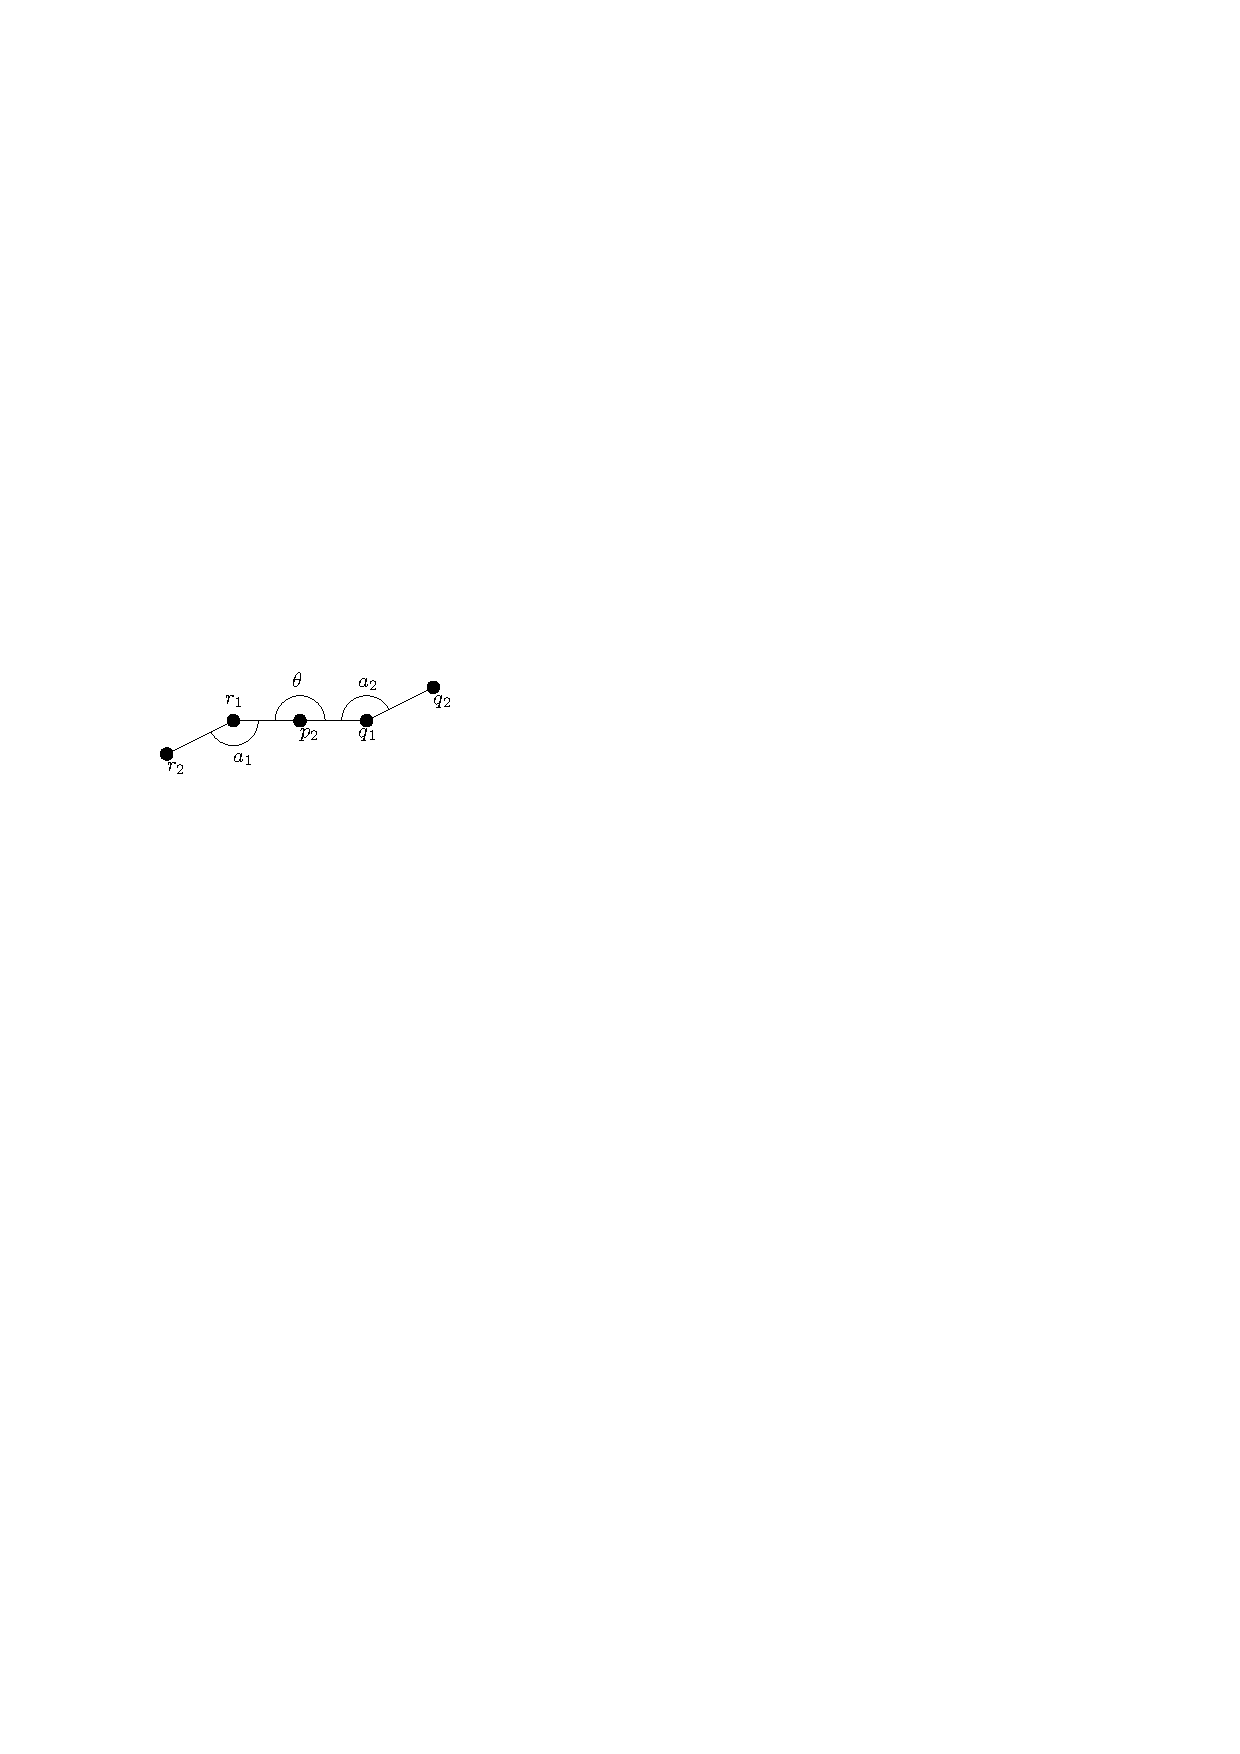
\includegraphics[width=0.5\linewidth]{NetworkRemoveSegmentsDetail}
  \caption{Schematic of $\theta$, $\alpha_1$ and $\alpha_2$}
  \label{networkremove}
\end{figure}
  
$RN$ is now an unconnected graph. For $RN$ to represent the road network it must be connected. Points that are not connected have degree 1. $d_{max}$ is defined as the maximum distance that is allowed between two points for them to form a new segment. For every point $p_3 \in P$ that has degree 1, the 10 most nearest points are found. $q_3 \in P$ is the point such that $s_{q_3, p_3} \in S$. Let $p_{near} \in Adj_{p_3,10}$ be such a point and $\alpha_3=\varphi(s_{q_3, p_3},s_{p_3, p_{near}})$. If $\alpha_3>\alpha_{min}$, $d(p_3,p_{near})<d_{max}$ and $s_{p_3, p_{near}}$ does not intersect any other segment in $S$ then $S=S \cup \{s_{p_3, p_{near}}\}$. In case a intersection does occur at point $u_1 \in U$ with segment $s_{w_1, w_2}\in S$, $P_{add}=P_{add}\cup \{u\}$. Four new segments $s_{w_1, u_1}$, $s_{u_1, w_2}$, $s_{p_3, u_1}$ and $s_{u_1, p_{near}}$ are added to $S$ and $s_{w_1, w_2}$ is removed from $S$, see figure \ref{addintersect}.

\begin{figure}[h]
\centering
      \graphicspath{ {images/}}
      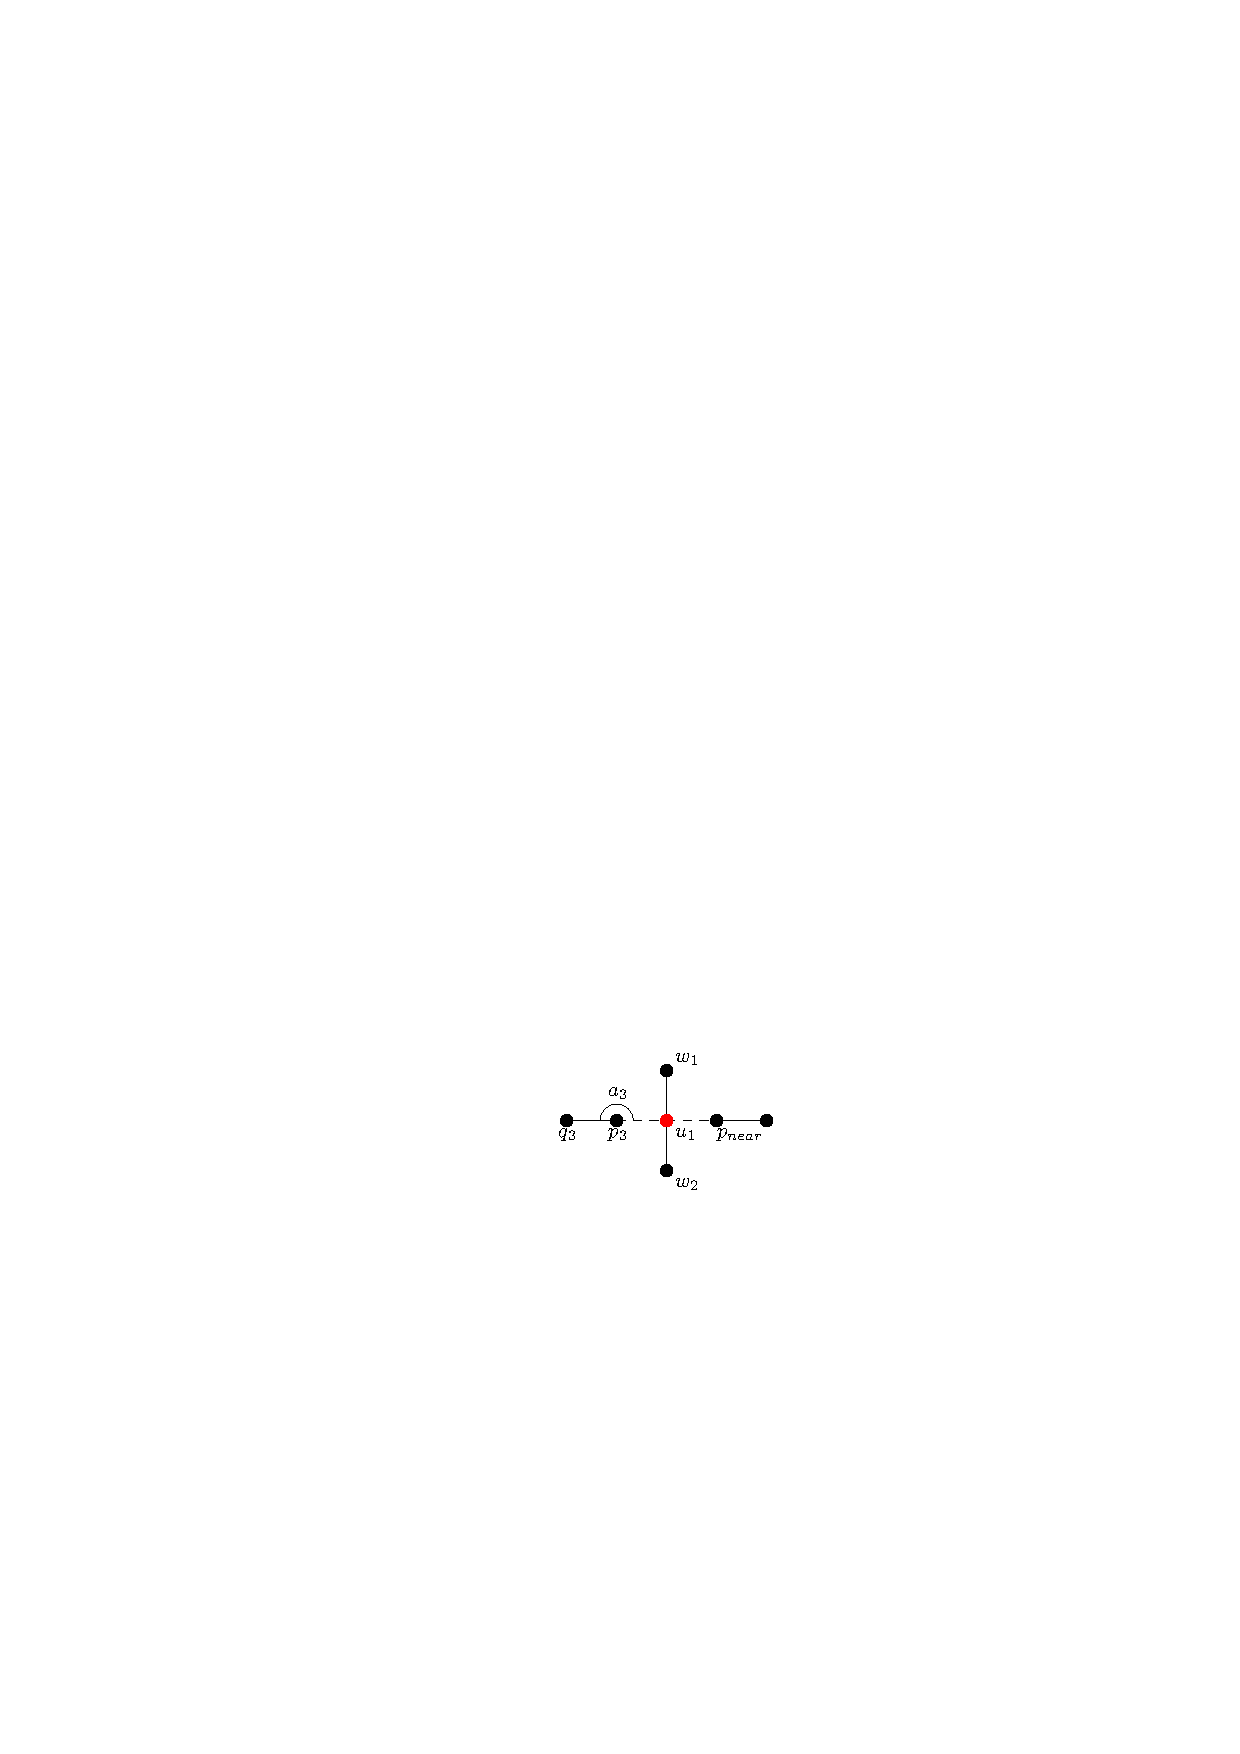
\includegraphics[width=0.5\linewidth]{NetworkAddIntersection}
      \caption{Adding a new segment that intersects the existing segment $s_{w_1,w_2}$}.
      \label{addintersect}
  \end{figure}

When no such point is found in $Adj_{p_3,10}$ the segment $s_{q_3, p_3}$ is extended, in the same direction, with a new segment $s_{p_3,q_4}$ where $q_4 \in U$ and $d(p_3,q_4)=d_{max}$. If $s_{p_3,q_4}$ intersects with another segment $s_{w_3,w_4} \in S$ at $u_2 \in U$ then three new segments $s_{p_3,u_2}$, $s_{w_3,u_2}$ and $s_{u_2,w_4}$ are added to $S$, $s_{w_3,w_4}$ is removed from $S$ and $P_{add}=P_{add}\cup \{u_2\}$. Every point with degree 1 is visited, in the worse case these are all points. For every point at most 10 points are looked up in the adjacency list. Comparisons between the points takes $O(1)$. This gives a running time of $O(n)$.

If we add the running times for each step that gives us: $O(n^2)+O(n)+O(n^2)+O(n)=O(n^2)$. The first step of the algorithm creates a minimum spanning tree that uses $O(n)$ storage. In the second step at most $n-1$ segments are added. The last step only creates a new segment if another segment is removed. The adjacency lists take $O(mn)$ storage, where $m$ is the number of nearby points to store. Since this is a constant the adjacency lists use $O(n)$ storage. Combining these results gives a total storage of $O(n)$.


\section{Experimental evaluation}
\subsection{Generating input}
To properly test the presented algorithms, many test cases have been created. The majority of these test cases were created by hand, made to be as difficult as possible for the algorithms. Some have sharp corners, or have points with large gaps between them as shown in figure \ref{single}.

\begin{figure}[ht!]
\centering
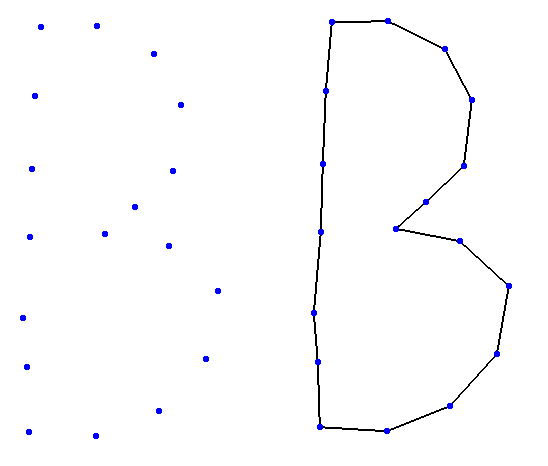
\includegraphics[scale=0.2]{anglesamplerate.png}
\caption{Test case with low sampling and a sharp angle (left) and the resulting output from the single curve algorithm (right.)}
\label{single}
\end{figure}

Other test cases have been created to test the running time of the algorithm, with the amount of nodes ranging from $100$ to $10000$. This same input is then used on all algorithms.

\begin{table}[ht!]
    \begin{tabular}{lrrrrr}
    ~                       & 100 nodes & 500 nodes & 1.000 nodes & 5.000 			nodes & 10.000 nodes \\
    Single Reconstruction   & 33ms      & 126ms     & 782ms       & 3.985ms     	& 20.604ms     \\
    Multiple Reconstruction & 38ms      & 146ms     & 207ms       & 2.947ms     	& 7.387ms      \\
    Network Reconstruction  & 18ms      & 85ms      & 143ms       & 1.996ms     	& 4.802ms      \\
    \end{tabular}
\caption{Table showing the computing time required for different input sizes.}
\end{table}

The multiple curve algorithm has additional test cases that are not run by the single curve algorithm, made specifically to test whether it correctly distinguishes between the multiple curves. These include curves enclosed in another curve, some curves that are close to each other and multiple curves that spiral around each other, some examples of these test cases are given in figure \ref{multi}.

\begin{figure}[ht!]
\centering
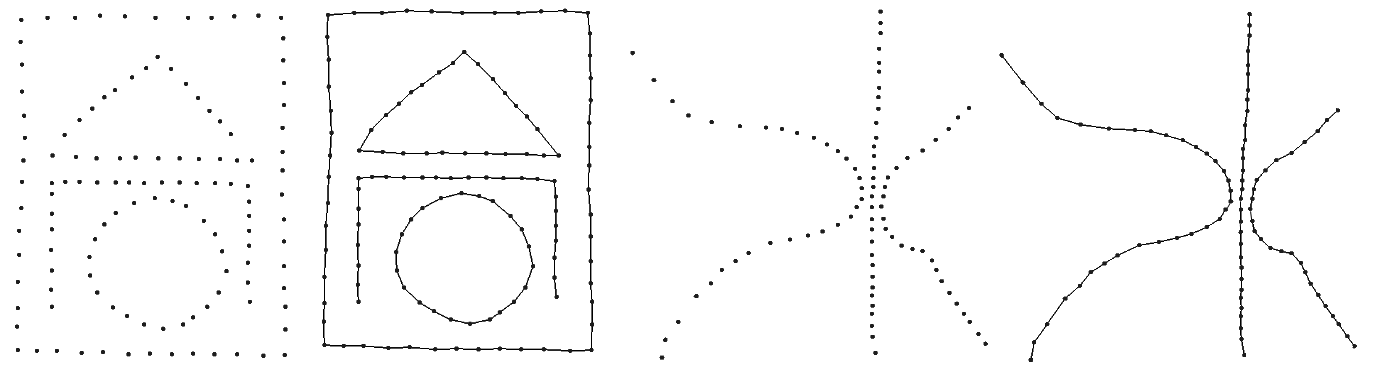
\includegraphics[scale=0.3]{multiInput.png}
\caption{A collection of test cases specifically for the multiple curve algorithm, with the correct output displayed to the right of it.}
\label{multi}
\end{figure}

The network algorithm has different input than the other two given curve reconstruction algorithms, so it therefore also requires specific test cases. For this, test cases have been modeled after real life road maps. Some test have also been created to test specific parts of the algorithm, for instance a inputs that has close parallel lines, merging roads and roundabouts.

\begin{figure}[ht!]
\centering
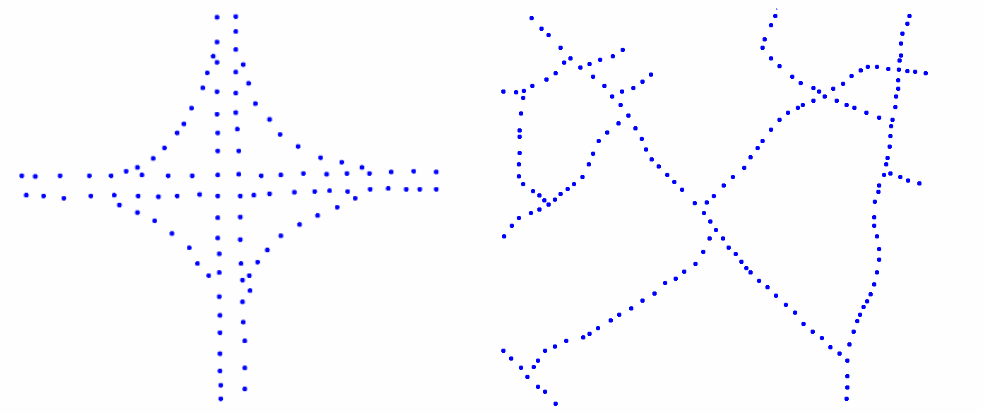
\includegraphics[scale=0.3]{networkInput.png}
\caption{A large intersection to test for parrallel and merging lines (Left) Simple neighbourhood (Right)}
\label{network}
\end{figure}$ $\\

\subsection{Resulting output}

\subsubsection{Single curve}
The single curve algorithm strongly depends on the ability of the likelihood function to accurately measuring how effective the resulting change would be. In the specifics of the algorithm, a segment is routinely removed and replaced by two new segments. This should contribute to a positive change in the curve. Clearly, the likelihood should increase when the two new segments are more like the old one. The triangle inequality gives the interesting opportunity to define the likelihood as follows, while taking into account the angle between the old segment and the new segments, as well as their variation in length:

\noindent
\begin{enumerate}
\topsep=0pt
\itemsep=0pt
\parsep=0pt
\item Ratio of squared segment lengths:\\
$s_{u,v} \in S \wedge p \in P \Rightarrow likelihood(s_{u,v}, p) = d(u, v)*d(u, v)/(d(p, v)*d(p, v)+d(p, u)*d(p, u))$
\item Ratio of segment lengths:\\
$s_{u,v} \in S \wedge p \in P \Rightarrow likelihood(s_{u,v}, p) = d(u, v)/(d(p, v)+d(p, u))$
\end{enumerate}

\begingroup
\tikzset{every picture/.style={scale=0.5,radius=0.05,line width=0.4}}%
\begin{figure}[ht!]
\centering
\begin{subfigure}{.24\linewidth}
\centering
%% Include the picture as follows: \
% \begingroup
% \tikzset{every picture/.style={scale=1,radius=0.05,line width=0.4}}%
% \input{tikz/[filename].tex}%
% \endgroup
%
%% Want to add a label? Use node[<position>]{label},
%% where <position> is one of: below / above / left / right
% \fill (0,0) circle node[below]{$p_1$};
%% Want to give the point a different color?
% \fill[red] (0,0) circle;
%
\begin{tikzpicture}
\draw (2.2171,7.0362) -- (2.1842,7.4474);
\draw (3.8454,2.6447) -- (3.6151,2.6118);
\draw (7.7928,3.2533) -- (7.7105,3.4013);
\draw (7.0033,3.3520) -- (7.1513,3.5493);
\draw (7.7928,3.2533) -- (7.9079,3.3520);
\draw (1.4112,7.5954) -- (1.2138,7.7434);
\draw (2.5789,7.6283) -- (2.3158,7.6118);
\draw (4.5855,8.7303) -- (4.8816,8.7467);
\draw (6.0329,4.6842) -- (6.0329,4.8980);
\draw (6.0329,4.6842) -- (6.0822,4.4868);
\draw (4.0592,4.1250) -- (3.9770,4.2237);
\draw (2.0855,7.1678) -- (1.9539,7.0526);
\draw (2.0855,7.1678) -- (1.8388,7.2007);
\draw (4.0921,2.6447) -- (4.2895,2.6447);
\draw (8.1546,3.2862) -- (8.0066,3.4013);
\draw (4.0592,4.1250) -- (4.2072,3.8454);
\draw (3.2039,7.1020) -- (3.0230,7.0526);
\draw (9.2401,2.9079) -- (9.0428,2.9079);
\draw (5.0461,2.4638) -- (5.0625,2.6118);
\draw (4.0921,2.6447) -- (3.8454,2.6447);
\draw (1.2138,7.7434) -- (1.3289,7.9901);
\draw (5.0461,2.4638) -- (4.9967,2.3158);
\draw (5.7368,6.9539) -- (5.8684,6.8553);
\draw (6.0493,3.0066) -- (5.7862,3.0395);
\draw (2.2993,6.6086) -- (2.1349,6.6086);
\draw (6.5263,3.6645) -- (6.3783,3.8454);
\draw (2.2993,6.6086) -- (2.4474,6.6086);
\draw (5.7368,6.9539) -- (5.6711,7.2007);
\draw (3.6316,6.1151) -- (3.5493,6.3289);
\draw (4.0757,2.3651) -- (4.3224,2.3816);
\draw (4.8816,8.7467) -- (5.0461,8.6480);
\draw (4.5526,2.3980) -- (4.3224,2.3816);
\draw (5.9836,5.0789) -- (6.0329,4.8980);
\draw (3.6316,6.1151) -- (3.6316,5.9178);
\draw (8.1546,2.8586) -- (8.3026,2.8586);
\draw (2.2171,7.0362) -- (2.2993,7.1513);
\draw (3.3026,7.2007) -- (3.2039,7.1020);
\draw (8.7796,3.3191) -- (8.8947,3.1546);
\draw (3.2204,8.0724) -- (2.8914,8.0888);
\draw (6.0493,3.0066) -- (6.2961,2.9901);
\draw (3.2204,8.0724) -- (3.4671,8.0724);
\draw (7.9079,3.3520) -- (8.0066,3.4013);
\draw (5.8355,6.4276) -- (6.0164,6.3783);
\draw (5.8355,6.4276) -- (5.9507,6.5592);
\draw (8.8125,2.9079) -- (9.0428,2.9079);
\draw (3.7632,2.3487) -- (3.5658,2.3487);
\draw (2.3158,7.6118) -- (2.0526,7.5954);
\draw (1.3289,7.9901) -- (1.4934,8.1546);
\draw (2.1349,6.6086) -- (1.8553,6.6086);
\draw (8.2368,3.1711) -- (8.1546,3.2862);
\draw (6.0329,6.8059) -- (5.8684,6.8553);
\draw (8.7796,3.3191) -- (8.6151,3.1711);
\draw (8.1546,2.8586) -- (7.9572,2.8586);
\draw (5.0954,8.4507) -- (5.0789,8.2039);
\draw (3.7632,2.3487) -- (4.0757,2.3651);
\draw (3.5493,6.3289) -- (3.3849,6.4770);
\draw (3.8783,4.3882) -- (3.7796,4.6842);
\draw (3.8783,4.3882) -- (3.9770,4.2237);
\draw (3.3849,7.2829) -- (3.3026,7.2007);
\draw (3.3849,7.2829) -- (3.3849,7.4803);
\draw (7.7105,3.4013) -- (7.5789,3.5000);
\draw (4.5033,2.7928) -- (4.5691,2.9901);
\draw (4.5033,2.7928) -- (4.2895,2.6447);
\draw (3.4671,8.0724) -- (3.8125,8.1053);
\draw (5.1118,2.9079) -- (5.0625,2.6118);
\draw (5.9178,5.7862) -- (6.0164,6.0000);
\draw (8.6645,2.9079) -- (8.5164,2.9079);
\draw (2.5461,7.1513) -- (2.4474,7.4474);
\draw (3.5658,2.3487) -- (3.3026,2.4145);
\draw (2.1842,7.4474) -- (1.9046,7.4474);
\draw (4.7500,2.3487) -- (4.9967,2.3158);
\draw (8.4013,3.3520) -- (8.5329,3.2533);
\draw (5.5888,3.1546) -- (5.7862,3.0395);
\draw (1.5757,7.0855) -- (1.4605,7.0362);
\draw (7.0033,3.3520) -- (6.9211,3.5329);
\draw (3.2697,7.5789) -- (3.1217,7.6612);
\draw (1.5757,7.0855) -- (1.6743,7.2171);
\draw (7.6941,2.8257) -- (7.9572,2.8586);
\draw (5.0954,8.4507) -- (5.0461,8.6480);
\draw (2.4803,7.0362) -- (2.5461,7.1513);
\draw (2.4803,7.0362) -- (2.2993,7.1513);
\draw (3.7796,4.6842) -- (3.7303,4.9803);
\draw (3.3849,7.4803) -- (3.2697,7.5789);
\draw (7.4638,3.3849) -- (7.5789,3.5000);
\draw (7.4803,2.8421) -- (7.3158,2.9079);
\draw (8.3026,2.8586) -- (8.5164,2.9079);
\draw (7.4803,2.8421) -- (7.6941,2.8257);
\draw (8.6151,3.1711) -- (8.5329,3.2533);
\draw (2.0526,7.5954) -- (1.7401,7.6118);
\draw (3.3026,2.4145) -- (3.1711,2.4967);
\draw (4.5526,2.3980) -- (4.7500,2.3487);
\draw (1.7401,8.1546) -- (1.4934,8.1546);
\draw (1.7072,6.6086) -- (1.8553,6.6086);
\draw (5.3586,3.2368) -- (5.5888,3.1546);
\draw (3.2368,6.5921) -- (2.9737,6.5921);
\draw (3.1217,7.6612) -- (2.6776,7.4474);
\draw (3.2368,6.5921) -- (3.3849,6.4770);
\draw (5.9178,5.7862) -- (6.0493,5.6711);
\draw (4.0757,8.2204) -- (4.2072,8.4342);
\draw (9.3553,2.9079) -- (9.2401,2.9079);
\draw (7.2664,3.4013) -- (7.1513,3.5493);
\draw (6.1316,6.7072) -- (6.0329,6.8059);
\draw (4.5691,3.2862) -- (4.5691,2.9901);
\draw (1.7401,8.1546) -- (2.0855,8.1217);
\draw (4.0757,8.2204) -- (3.8125,8.1053);
\draw (6.1316,6.7072) -- (5.9507,6.5592);
\draw (5.9836,5.0789) -- (6.0658,5.2763);
\draw (4.3059,3.7303) -- (4.4211,3.5493);
\draw (1.4605,6.6579) -- (1.3454,6.7401);
\draw (6.1645,5.4408) -- (6.2138,5.5724);
\draw (5.1941,3.2533) -- (5.1447,3.1217);
\draw (4.3059,3.7303) -- (4.2072,3.8454);
\draw (1.4605,6.6579) -- (1.7072,6.6086);
\draw (5.1941,3.2533) -- (5.3586,3.2368);
\draw (2.8586,7.1678) -- (2.9408,7.4967);
\draw (7.3651,3.2697) -- (7.4638,3.3849);
\draw (1.7730,7.0526) -- (1.6743,7.2171);
\draw (7.3651,3.2697) -- (7.2664,3.4013);
\draw (5.1447,8.0066) -- (5.0789,8.2039);
\draw (5.1447,8.0066) -- (5.3257,7.8257);
\draw (3.6645,5.2105) -- (3.6645,5.4572);
\draw (6.9211,3.5329) -- (6.8059,3.6809);
\draw (3.6645,5.2105) -- (3.7303,4.9803);
\draw (4.5691,3.4342) -- (4.5691,3.2862);
\draw (6.9704,2.9079) -- (6.7895,2.9408);
\draw (6.9704,2.9079) -- (7.3158,2.9079);
\draw (8.8947,3.1546) -- (9.0921,3.1053);
\draw (4.5691,3.4342) -- (4.4211,3.5493);
\draw (2.7434,7.0362) -- (2.8586,7.1678);
\draw (1.3454,6.7401) -- (1.3125,6.9046);
\draw (1.7401,7.6118) -- (1.5921,7.4309);
\draw (3.3684,2.6118) -- (3.1711,2.4967);
\draw (3.3684,2.6118) -- (3.6151,2.6118);
\draw (6.5263,3.6645) -- (6.8059,3.6809);
\draw (2.6283,6.6250) -- (2.7763,6.6086);
\draw (2.6283,6.6250) -- (2.4474,6.6086);
\draw (5.4243,7.6612) -- (5.5888,7.4638);
\draw (5.1447,3.1217) -- (5.1118,2.9079);
\draw (2.8257,7.6612) -- (2.5789,7.6283);
\draw (5.4243,7.6612) -- (5.3257,7.8257);
\draw (6.3783,3.8454) -- (6.2796,4.0099);
\draw (4.3882,8.5822) -- (4.2072,8.4342);
\draw (1.4605,7.0362) -- (1.3125,6.9046);
\draw (1.9046,7.4474) -- (1.8388,7.2007);
\draw (9.2730,3.0559) -- (9.5362,2.9243);
\draw (9.2730,3.0559) -- (9.0921,3.1053);
\draw (2.3322,8.1053) -- (2.0855,8.1217);
\draw (6.1645,5.4408) -- (6.0658,5.2763);
\draw (6.0493,5.6711) -- (6.2138,5.5724);
\draw (1.5921,7.4309) -- (1.4112,7.5954);
\draw (5.5888,7.4638) -- (5.6711,7.2007);
\draw (2.7763,6.6086) -- (2.9737,6.5921);
\draw (2.6776,7.4474) -- (2.4474,7.4474);
\draw (8.2368,3.1711) -- (8.4013,3.3520);
\draw (6.1480,4.2237) -- (6.2796,4.0099);
\draw (8.6645,2.9079) -- (8.8125,2.9079);
\draw (4.4868,8.6645) -- (4.5855,8.7303);
\draw (3.6316,5.6053) -- (3.6645,5.4572);
\draw (6.1480,4.2237) -- (6.0822,4.4868);
\draw (3.6316,5.6053) -- (3.6316,5.9178);
\draw (1.9539,7.0526) -- (1.7730,7.0526);
\draw (4.4868,8.6645) -- (4.3882,8.5822);
\draw (6.5428,2.9572) -- (6.2961,2.9901);
\draw (2.6776,8.1217) -- (2.8914,8.0888);
\draw (6.5428,2.9572) -- (6.7895,2.9408);
\draw (6.1480,6.2632) -- (6.0164,6.3783);
\draw (9.3553,2.9079) -- (9.5362,2.9243);
\draw (6.1480,6.2632) -- (6.0164,6.0000);
\draw (2.6776,8.1217) -- (2.3322,8.1053);
\draw (3.0230,7.0526) -- (2.7434,7.0362);
\fill (1.3125,6.9046) circle;
\fill (1.3454,6.7401) circle;
\fill (1.4605,6.6579) circle;
\fill (1.7072,6.6086) circle;
\fill (1.8553,6.6086) circle;
\fill (2.1349,6.6086) circle;
\fill (2.2993,6.6086) circle;
\fill (2.4474,6.6086) circle;
\fill (2.7763,6.6086) circle;
\fill (2.6283,6.6250) circle;
\fill (2.9737,6.5921) circle;
\fill (3.2368,6.5921) circle;
\fill (3.3849,6.4770) circle;
\fill (3.5493,6.3289) circle;
\fill (3.6316,6.1151) circle;
\fill (3.6316,5.9178) circle;
\fill (3.6316,5.6053) circle;
\fill (3.6645,5.4572) circle;
\fill (3.6645,5.2105) circle;
\fill (3.7303,4.9803) circle;
\fill (3.7796,4.6842) circle;
\fill (3.8783,4.3882) circle;
\fill (3.9770,4.2237) circle;
\fill (4.0592,4.1250) circle;
\fill (4.2072,3.8454) circle;
\fill (4.4211,3.5493) circle;
\fill (4.5691,3.4342) circle;
\fill (4.5691,3.2862) circle;
\fill (4.5691,2.9901) circle;
\fill (4.5033,2.7928) circle;
\fill (4.2895,2.6447) circle;
\fill (4.0921,2.6447) circle;
\fill (3.8454,2.6447) circle;
\fill (3.6151,2.6118) circle;
\fill (3.3684,2.6118) circle;
\fill (3.1711,2.4967) circle;
\fill (3.3026,2.4145) circle;
\fill (3.5658,2.3487) circle;
\fill (3.7632,2.3487) circle;
\fill (4.0757,2.3651) circle;
\fill (4.3224,2.3816) circle;
\fill (5.1118,2.9079) circle;
\fill (5.1447,3.1217) circle;
\fill (5.1941,3.2533) circle;
\fill (5.3586,3.2368) circle;
\fill (5.5888,3.1546) circle;
\fill (5.7862,3.0395) circle;
\fill (6.0493,3.0066) circle;
\fill (6.2961,2.9901) circle;
\fill (6.5428,2.9572) circle;
\fill (6.7895,2.9408) circle;
\fill (6.9704,2.9079) circle;
\fill (7.3158,2.9079) circle;
\fill (7.4803,2.8421) circle;
\fill (7.6941,2.8257) circle;
\fill (8.1546,2.8586) circle;
\fill (8.3026,2.8586) circle;
\fill (8.6645,2.9079) circle;
\fill (8.8125,2.9079) circle;
\fill (9.2401,2.9079) circle;
\fill (9.3553,2.9079) circle;
\fill (9.2730,3.0559) circle;
\fill (8.8947,3.1546) circle;
\fill (8.7796,3.3191) circle;
\fill (8.6151,3.1711) circle;
\fill (8.4013,3.3520) circle;
\fill (8.2368,3.1711) circle;
\fill (8.0066,3.4013) circle;
\fill (7.7928,3.2533) circle;
\fill (7.5789,3.5000) circle;
\fill (7.9572,2.8586) circle;
\fill (7.3651,3.2697) circle;
\fill (7.1513,3.5493) circle;
\fill (7.0033,3.3520) circle;
\fill (6.8059,3.6809) circle;
\fill (6.5263,3.6645) circle;
\fill (6.2796,4.0099) circle;
\fill (6.0822,4.4868) circle;
\fill (6.0329,4.8980) circle;
\fill (5.9178,5.7862) circle;
\fill (5.8355,6.4276) circle;
\fill (6.0164,6.0000) circle;
\fill (6.1480,6.2632) circle;
\fill (6.0164,6.3783) circle;
\fill (5.9507,6.5592) circle;
\fill (6.1316,6.7072) circle;
\fill (5.8684,6.8553) circle;
\fill (6.0329,6.8059) circle;
\fill (5.7368,6.9539) circle;
\fill (5.6711,7.2007) circle;
\fill (5.5888,7.4638) circle;
\fill (5.4243,7.6612) circle;
\fill (5.1447,8.0066) circle;
\fill (5.3257,7.8257) circle;
\fill (5.0789,8.2039) circle;
\fill (5.0954,8.4507) circle;
\fill (5.0461,8.6480) circle;
\fill (4.8816,8.7467) circle;
\fill (4.5855,8.7303) circle;
\fill (4.4868,8.6645) circle;
\fill (4.3882,8.5822) circle;
\fill (4.2072,8.4342) circle;
\fill (4.0757,8.2204) circle;
\fill (3.8125,8.1053) circle;
\fill (3.4671,8.0724) circle;
\fill (3.2204,8.0724) circle;
\fill (2.8914,8.0888) circle;
\fill (2.6776,8.1217) circle;
\fill (2.3322,8.1053) circle;
\fill (2.0855,8.1217) circle;
\fill (1.7401,8.1546) circle;
\fill (1.4934,8.1546) circle;
\fill (1.3289,7.9901) circle;
\fill (1.2138,7.7434) circle;
\fill (1.4112,7.5954) circle;
\fill (1.5921,7.4309) circle;
\fill (1.7401,7.6118) circle;
\fill (1.9046,7.4474) circle;
\fill (2.0526,7.5954) circle;
\fill (2.1842,7.4474) circle;
\fill (2.3158,7.6118) circle;
\fill (2.4474,7.4474) circle;
\fill (2.5789,7.6283) circle;
\fill (2.6776,7.4474) circle;
\fill (2.8257,7.6612) circle;
\fill (2.9408,7.4967) circle;
\fill (3.1217,7.6612) circle;
\fill (3.2697,7.5789) circle;
\fill (3.3849,7.4803) circle;
\fill (3.3849,7.2829) circle;
\fill (3.3026,7.2007) circle;
\fill (3.2039,7.1020) circle;
\fill (3.0230,7.0526) circle;
\fill (2.8586,7.1678) circle;
\fill (2.7434,7.0362) circle;
\fill (2.5461,7.1513) circle;
\fill (2.4803,7.0362) circle;
\fill (2.2993,7.1513) circle;
\fill (2.2171,7.0362) circle;
\fill (2.0855,7.1678) circle;
\fill (1.9539,7.0526) circle;
\fill (1.8388,7.2007) circle;
\fill (1.7730,7.0526) circle;
\fill (1.6743,7.2171) circle;
\fill (1.5757,7.0855) circle;
\fill (1.4605,7.0362) circle;
\fill (4.3059,3.7303) circle;
\fill (8.5164,2.9079) circle;
\fill (9.0428,2.9079) circle;
\fill (9.0921,3.1053) circle;
\fill (9.5362,2.9243) circle;
\fill (4.5526,2.3980) circle;
\fill (4.7500,2.3487) circle;
\fill (4.9967,2.3158) circle;
\fill (5.0461,2.4638) circle;
\fill (5.0625,2.6118) circle;
\fill (6.0493,5.6711) circle;
\fill (6.2138,5.5724) circle;
\fill (6.1645,5.4408) circle;
\fill (6.0658,5.2763) circle;
\fill (5.9836,5.0789) circle;
\fill (6.0329,4.6842) circle;
\fill (6.1480,4.2237) circle;
\fill (6.3783,3.8454) circle;
\fill (6.9211,3.5329) circle;
\fill (7.2664,3.4013) circle;
\fill (7.4638,3.3849) circle;
\fill (7.7105,3.4013) circle;
\fill (7.9079,3.3520) circle;
\fill (8.1546,3.2862) circle;
\fill (8.5329,3.2533) circle;
\end{tikzpicture}

\label{fig:exp:single_parameter_a:first}
\end{subfigure}%
\begin{subfigure}{.24\linewidth}
\centering
%% Include the picture as follows: \
% \begingroup
% \tikzset{every picture/.style={scale=1,radius=0.05,line width=0.4}}%
% \input{tikz/[filename].tex}%
% \endgroup
%
%% Want to add a label? Use node[<position>]{label},
%% where <position> is one of: below / above / left / right
% \fill (0,0) circle node[below]{$p_1$};
%% Want to give the point a different color?
% \fill[red] (0,0) circle;
%
\begin{tikzpicture}
\draw (3.7467,1.6414) -- (2.4967,1.7072);
\draw (4.0099,2.6447) -- (3.7467,1.6414);
\draw (3.9112,3.4178) -- (4.0099,2.6447);
\draw (4.1908,4.1579) -- (3.9112,3.4178);
\draw (2.9572,2.6118) -- (2.4967,1.7072);
\draw (6.5099,4.9967) -- (6.7072,4.1086);
\draw (5.0954,3.8783) -- (6.7072,4.1086);
\draw (4.1908,4.1579) -- (5.0954,3.8783);
\draw (5.0296,7.7599) -- (4.9309,6.9704);
\draw (5.1283,4.7500) -- (6.5099,4.9967);
\draw (5.1941,6.0000) -- (4.9309,6.9704);
\draw (5.1283,4.7500) -- (5.1941,6.0000);
\draw (4.7171,9.7500) -- (5.1776,9.2401);
\draw (4.7336,8.5493) -- (5.1776,9.2401);
\draw (3.7961,9.7500) -- (4.7171,9.7500);
\draw (4.7336,8.5493) -- (5.0296,7.7599);
\draw (2.7105,3.2697) -- (2.9408,3.9770);
\draw (3.5164,8.1875) -- (3.4013,9.2072);
\draw (3.4013,9.2072) -- (3.7961,9.7500);
\draw (2.7105,3.2697) -- (2.9572,2.6118);
\draw (3.3520,5.3092) -- (2.9408,3.9770);
\draw (3.3520,5.3092) -- (3.0724,6.6086);
\draw (3.5164,8.1875) -- (3.0724,6.6086);
\fill (2.4967,1.7072) circle;
\fill (3.7467,1.6414) circle;
\fill (4.0099,2.6447) circle;
\fill (3.9112,3.4178) circle;
\fill (4.1908,4.1579) circle;
\fill (5.0954,3.8783) circle;
\fill (6.7072,4.1086) circle;
\fill (6.5099,4.9967) circle;
\fill (5.1283,4.7500) circle;
\fill (5.1941,6.0000) circle;
\fill (4.9309,6.9704) circle;
\fill (5.0296,7.7599) circle;
\fill (4.7336,8.5493) circle;
\fill (5.1776,9.2401) circle;
\fill (4.7171,9.7500) circle;
\fill (3.7961,9.7500) circle;
\fill (3.4013,9.2072) circle;
\fill (3.5164,8.1875) circle;
\fill (3.3520,5.3092) circle;
\fill (3.0724,6.6086) circle;
\fill (2.9408,3.9770) circle;
\fill (2.7105,3.2697) circle;
\fill (2.9572,2.6118) circle;
\end{tikzpicture}

\label{fig:exp:single_parameter_a:second}
\centering
\end{subfigure}
\begin{subfigure}{.24\linewidth}
\centering
reconstruct single
171 number of sample points
1 0.13125 0.69046056
2 0.13453947 0.6740132
3 0.14605263 0.6657895
4 0.17072368 0.6608553
5 0.18552631 0.6608553
6 0.21348684 0.6608553
7 0.22993422 0.6608553
8 0.24473682 0.6608553
9 0.27763158 0.6608553
10 0.26282895 0.6625
11 0.29736844 0.65921056
12 0.32368422 0.65921056
13 0.33848685 0.64769745
14 0.35493422 0.63289475
15 0.3631579 0.6115132
16 0.3631579 0.5917764
17 0.3631579 0.5605263
18 0.36644736 0.54572374
19 0.36644736 0.52105266
20 0.37302634 0.49802628
21 0.37796053 0.46842104
22 0.38782895 0.4388158
23 0.3976974 0.42236844
24 0.40592107 0.4125
25 0.42072368 0.38453946
26 0.44210526 0.35493422
27 0.45690787 0.34342104
28 0.45690787 0.3286184
29 0.45690787 0.29901317
30 0.45032895 0.2792763
31 0.4289474 0.26447368
32 0.40921053 0.26447368
33 0.38453946 0.26447368
34 0.36151317 0.26118422
35 0.3368421 0.26118422
36 0.31710526 0.24967107
37 0.33026317 0.24144739
38 0.35657895 0.2348684
39 0.37631577 0.2348684
40 0.40756577 0.23651314
41 0.43223682 0.2381579
42 0.5111842 0.29078948
43 0.5144737 0.31217104
44 0.5194079 0.32532895
45 0.5358553 0.32368422
46 0.5588816 0.31546053
47 0.57861847 0.30394736
48 0.6049342 0.30065787
49 0.6296053 0.29901317
50 0.6542763 0.29572368
51 0.6789474 0.29407895
52 0.69703954 0.29078948
53 0.731579 0.29078948
54 0.7480264 0.2842105
55 0.7694079 0.2825658
56 0.81546056 0.28585526
57 0.8302632 0.28585526
58 0.8664474 0.29078948
59 0.88125 0.29078948
60 0.9240132 0.29078948
61 0.9355264 0.29078948
62 0.9273027 0.30559212
63 0.8894737 0.31546053
64 0.87796056 0.3319079
65 0.8615132 0.31710526
66 0.8401316 0.33519736
67 0.8236842 0.31710526
68 0.8006579 0.34013158
69 0.7792764 0.32532895
70 0.75789475 0.35
71 0.79572374 0.28585526
72 0.7365132 0.32697368
73 0.71513164 0.35493422
74 0.70032895 0.33519736
75 0.6805922 0.3680921
76 0.65263164 0.36644736
77 0.62796056 0.40098682
78 0.60822374 0.4486842
79 0.60328954 0.48980263
80 0.5917764 0.57861847
81 0.58355266 0.64276314
82 0.60164475 0.6
83 0.6148027 0.6263158
84 0.60164475 0.63782895
85 0.59506583 0.6559211
86 0.6131579 0.6707237
87 0.5868421 0.6855264
88 0.60328954 0.6805922
89 0.5736843 0.69539475
90 0.5671053 0.72006583
91 0.5588816 0.74638164
92 0.5424342 0.7661184
93 0.5144737 0.8006579
94 0.53256583 0.7825658
95 0.5078948 0.8203948
96 0.5095395 0.84506583
97 0.5046053 0.86480266
98 0.4881579 0.8746711
99 0.45855263 0.8730263
100 0.4486842 0.8664474
101 0.4388158 0.85822374
102 0.42072368 0.8434211
103 0.40756577 0.8220395
104 0.38125002 0.8105263
105 0.34671053 0.80723685
106 0.32203948 0.80723685
107 0.28914475 0.80888164
108 0.26776314 0.8121711
109 0.23322368 0.8105263
110 0.20855263 0.8121711
111 0.17401317 0.81546056
112 0.1493421 0.81546056
113 0.13289474 0.79901314
114 0.12138157 0.7743421
115 0.14111842 0.75953954
116 0.15921052 0.7430922
117 0.17401317 0.7611842
118 0.19046053 0.74473685
119 0.20526315 0.75953954
120 0.21842106 0.74473685
121 0.23157895 0.7611842
122 0.24473682 0.74473685
123 0.25789475 0.762829
124 0.26776314 0.74473685
125 0.2825658 0.7661184
126 0.29407895 0.74967104
127 0.31217104 0.7661184
128 0.32697368 0.75789475
129 0.33848685 0.7480264
130 0.33848685 0.7282895
131 0.33026317 0.72006583
132 0.32039472 0.7101974
133 0.30230263 0.7052632
134 0.28585526 0.7167763
135 0.27434212 0.70361847
136 0.25460526 0.71513164
137 0.24802631 0.70361847
138 0.22993422 0.71513164
139 0.22171052 0.70361847
140 0.20855263 0.7167763
141 0.19539472 0.7052632
142 0.18388157 0.72006583
143 0.17730263 0.7052632
144 0.1674342 0.72171056
145 0.15756579 0.70855266
146 0.14605263 0.70361847
147 0.43059212 0.37302634
148 0.85164475 0.29078948
149 0.9042764 0.29078948
150 0.90921056 0.3105263
151 0.95361847 0.2924342
152 0.45526317 0.23980263
153 0.475 0.2348684
154 0.49967107 0.23157895
155 0.5046053 0.24638158
156 0.50625 0.26118422
157 0.6049342 0.5671053
158 0.6213816 0.5572369
159 0.6164474 0.54407895
160 0.606579 0.5276316
161 0.5983553 0.5078948
162 0.60328954 0.46842104
163 0.6148027 0.42236844
164 0.63782895 0.38453946
165 0.6921053 0.35328948
166 0.72664475 0.34013158
167 0.74638164 0.33848685
168 0.7710527 0.34013158
169 0.7907895 0.33519736
170 0.81546056 0.3286184
171 0.85328954 0.32532895

\label{fig:exp:single_parameter_a:third}
\end{subfigure}%
\begin{subfigure}{.24\linewidth}
\centering
%% Include the picture as follows: \
% \begingroup
% \tikzset{every picture/.style={scale=1,radius=0.05,line width=0.4}}%
% \input{tikz/[filename].tex}%
% \endgroup
%
%% Want to add a label? Use node[<position>]{label},
%% where <position> is one of: below / above / left / right
% \fill (0,0) circle node[below]{$p_1$};
%% Want to give the point a different color?
% \fill[red] (0,0) circle;
%
\begin{tikzpicture}
\draw (3.7467,1.6414) -- (2.4967,1.7072);
\draw (4.0099,2.6447) -- (3.7467,1.6414);
\draw (3.9112,3.4178) -- (4.0099,2.6447);
\draw (4.1908,4.1579) -- (3.9112,3.4178);
\draw (2.9572,2.6118) -- (2.4967,1.7072);
\draw (6.5099,4.9967) -- (6.7072,4.1086);
\draw (4.1908,4.1579) -- (5.0954,3.8783);
\draw (5.1283,4.7500) -- (6.7072,4.1086);
\draw (5.1283,4.7500) -- (5.0954,3.8783);
\draw (5.1941,6.0000) -- (6.5099,4.9967);
\draw (5.1941,6.0000) -- (4.9309,6.9704);
\draw (4.7171,9.7500) -- (5.1776,9.2401);
\draw (4.7336,8.5493) -- (5.1776,9.2401);
\draw (3.7961,9.7500) -- (4.7171,9.7500);
\draw (4.9309,6.9704) -- (5.0296,7.7599);
\draw (4.7336,8.5493) -- (5.0296,7.7599);
\draw (3.5164,8.1875) -- (3.4013,9.2072);
\draw (2.9572,2.6118) -- (2.7105,3.2697);
\draw (3.4013,9.2072) -- (3.7961,9.7500);
\draw (2.9408,3.9770) -- (2.7105,3.2697);
\draw (3.3520,5.3092) -- (2.9408,3.9770);
\draw (3.5164,8.1875) -- (3.0724,6.6086);
\draw (3.3520,5.3092) -- (3.0724,6.6086);
\fill (2.4967,1.7072) circle;
\fill (3.7467,1.6414) circle;
\fill (4.0099,2.6447) circle;
\fill (3.9112,3.4178) circle;
\fill (4.1908,4.1579) circle;
\fill (5.0954,3.8783) circle;
\fill (6.7072,4.1086) circle;
\fill (6.5099,4.9967) circle;
\fill (5.1283,4.7500) circle;
\fill (5.1941,6.0000) circle;
\fill (4.9309,6.9704) circle;
\fill (5.0296,7.7599) circle;
\fill (4.7336,8.5493) circle;
\fill (5.1776,9.2401) circle;
\fill (4.7171,9.7500) circle;
\fill (3.7961,9.7500) circle;
\fill (3.4013,9.2072) circle;
\fill (3.5164,8.1875) circle;
\fill (3.3520,5.3092) circle;
\fill (3.0724,6.6086) circle;
\fill (2.9408,3.9770) circle;
\fill (2.7105,3.2697) circle;
\fill (2.9572,2.6118) circle;
\end{tikzpicture}

\label{fig:exp:single_parameter_a:fourth}
\centering
\end{subfigure}
\caption{The solutions for two inputs, using squared segment lengths (left) and segment lengths (right) for the likelihood function ($k = 1.4$)}
\end{figure}
\endgroup

In addition, there exists the parameter $k$ so that a segment $s$ is deemed comparatively long in $S$ if $s = l1(S) \wedge l1(S) \geq k \cdot l2(S)$. Therefore $k$ may be chosen so that $1 < k$.

\begingroup
\tikzset{every picture/.style={scale=0.3,radius=0.05,line width=0.4}}%
\begin{figure}[ht!]
\centering
\begin{subfigure}{.15\linewidth}
\centering
%% Include the picture as follows: \
% \begingroup
% \tikzset{every picture/.style={scale=1,radius=0.05,line width=0.4}}%
% \input{tikz/[filename].tex}%
% \endgroup
%
%% Want to add a label? Use node[<position>]{label},
%% where <position> is one of: below / above / left / right
% \fill (0,0) circle node[below]{$p_1$};
%% Want to give the point a different color?
% \fill[red] (0,0) circle;
%
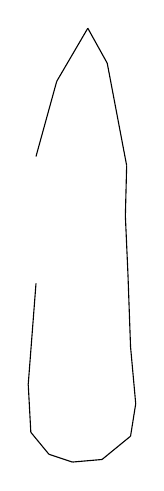
\begin{tikzpicture}
\draw (4.5033,8.8454) -- (4.7500,8.4013);
\draw (4.1086,8.1711) -- (4.5033,8.8454);
\draw (4.7500,8.4013) -- (4.9967,7.1020);
\draw (4.9803,6.4605) -- (4.9967,7.1020);
\draw (5.0461,4.7993) -- (5.0132,5.7204);
\draw (4.9803,6.4605) -- (5.0132,5.7204);
\draw (5.0461,4.7993) -- (5.1118,4.0757);
\draw (5.0461,3.6645) -- (4.6842,3.3684);
\draw (5.1118,4.0757) -- (5.0461,3.6645);
\draw (4.3059,3.3355) -- (4.0099,3.4342);
\draw (4.6842,3.3684) -- (4.3059,3.3355);
\draw (4.0099,3.4342) -- (3.7796,3.7138);
\draw (3.7796,3.7138) -- (3.7467,4.3224);
\draw (3.8454,5.6053) -- (3.7467,4.3224);
\draw (3.8454,7.2171) -- (4.1086,8.1711);
\fill (4.5033,8.8454) circle;
\fill (4.7500,8.4013) circle;
\fill (4.9967,7.1020) circle;
\fill (4.9803,6.4605) circle;
\fill (5.0132,5.7204) circle;
\fill (5.0461,4.7993) circle;
\fill (5.1118,4.0757) circle;
\fill (5.0461,3.6645) circle;
\fill (4.6842,3.3684) circle;
\fill (4.3059,3.3355) circle;
\fill (4.0099,3.4342) circle;
\fill (3.7796,3.7138) circle;
\fill (3.7467,4.3224) circle;
\fill (3.8454,5.6053) circle;
\fill (3.8454,7.2171) circle;
\fill (4.1086,8.1711) circle;
\end{tikzpicture}

\label{fig:exp:single_parameter_b:first}
\end{subfigure}%
\begin{subfigure}{.15\linewidth}
\centering
%% Include the picture as follows: \
% \begingroup
% \tikzset{every picture/.style={scale=1,radius=0.05,line width=0.4}}%
% \input{tikz/[filename].tex}%
% \endgroup
%
%% Want to add a label? Use node[<position>]{label},
%% where <position> is one of: below / above / left / right
% \fill (0,0) circle node[below]{$p_1$};
%% Want to give the point a different color?
% \fill[red] (0,0) circle;
%
\begin{tikzpicture}
\draw (1.7895,0.7270) -- (1.6908,1.8618);
\draw (2.7105,0.7105) -- (1.7895,0.7270);
\draw (1.6414,3.0625) -- (1.6908,1.8618);
\draw (1.5592,6.3191) -- (1.4934,5.5132);
\draw (1.6414,3.0625) -- (1.6086,4.1809);
\draw (1.5592,6.3191) -- (1.5921,7.3882);
\draw (2.6283,4.1480) -- (1.6086,4.1809);
\draw (2.6941,7.4539) -- (3.7303,7.0428);
\draw (1.5921,7.3882) -- (2.6941,7.4539);
\draw (3.8947,4.3289) -- (4.7007,5.0691);
\draw (4.5033,6.1875) -- (4.7007,5.0691);
\draw (3.7303,7.0428) -- (4.5033,6.1875);
\draw (3.3355,3.6875) -- (3.9605,3.0954);
\draw (3.3355,3.6875) -- (3.8947,4.3289);
\draw (3.6480,1.1711) -- (2.7105,0.7105);
\draw (3.9605,3.0954) -- (4.0921,2.0099);
\draw (4.0921,2.0099) -- (3.6480,1.1711);
\fill (1.7895,0.7270) circle;
\fill (1.6908,1.8618) circle;
\fill (1.6414,3.0625) circle;
\fill (1.6086,4.1809) circle;
\fill (1.4934,5.5132) circle;
\fill (1.5592,6.3191) circle;
\fill (1.5921,7.3882) circle;
\fill (2.6941,7.4539) circle;
\fill (3.7303,7.0428) circle;
\fill (4.5033,6.1875) circle;
\fill (4.7007,5.0691) circle;
\fill (3.8947,4.3289) circle;
\fill (2.6283,4.1480) circle;
\fill (3.3355,3.6875) circle;
\fill (3.9605,3.0954) circle;
\fill (4.0921,2.0099) circle;
\fill (3.6480,1.1711) circle;
\fill (2.7105,0.7105) circle;
\end{tikzpicture}

\label{fig:exp:single_parameter_b:second}
\centering
\end{subfigure}
\begin{subfigure}{.15\linewidth}
\centering
%% Include the picture as follows: \
% \begingroup
% \tikzset{every picture/.style={scale=1,radius=0.05,line width=0.4}}%
% \input{tikz/[filename].tex}%
% \endgroup
%
%% Want to add a label? Use node[<position>]{label},
%% where <position> is one of: below / above / left / right
% \fill (0,0) circle node[below]{$p_1$};
%% Want to give the point a different color?
% \fill[red] (0,0) circle;
%
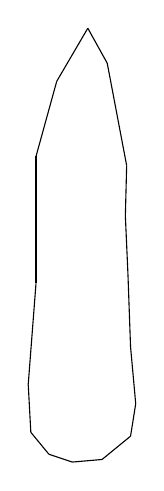
\begin{tikzpicture}
\draw (4.5033,8.8454) -- (4.7500,8.4013);
\draw (4.1086,8.1711) -- (4.5033,8.8454);
\draw (4.7500,8.4013) -- (4.9967,7.1020);
\draw (4.9803,6.4605) -- (4.9967,7.1020);
\draw (5.0461,4.7993) -- (5.0132,5.7204);
\draw (4.9803,6.4605) -- (5.0132,5.7204);
\draw (5.0461,4.7993) -- (5.1118,4.0757);
\draw (5.0461,3.6645) -- (4.6842,3.3684);
\draw (5.1118,4.0757) -- (5.0461,3.6645);
\draw (4.3059,3.3355) -- (4.0099,3.4342);
\draw (4.6842,3.3684) -- (4.3059,3.3355);
\draw (3.8454,5.6053) -- (3.8454,7.2171);
\draw (4.0099,3.4342) -- (3.7796,3.7138);
\draw (3.7796,3.7138) -- (3.7467,4.3224);
\draw (3.8454,5.6053) -- (3.7467,4.3224);
\draw (3.8454,7.2171) -- (4.1086,8.1711);
\fill (4.5033,8.8454) circle;
\fill (4.7500,8.4013) circle;
\fill (4.9967,7.1020) circle;
\fill (4.9803,6.4605) circle;
\fill (5.0132,5.7204) circle;
\fill (5.0461,4.7993) circle;
\fill (5.1118,4.0757) circle;
\fill (5.0461,3.6645) circle;
\fill (4.6842,3.3684) circle;
\fill (4.3059,3.3355) circle;
\fill (4.0099,3.4342) circle;
\fill (3.7796,3.7138) circle;
\fill (3.7467,4.3224) circle;
\fill (3.8454,5.6053) circle;
\fill (3.8454,7.2171) circle;
\fill (4.1086,8.1711) circle;
\end{tikzpicture}

\label{fig:exp:single_parameter_b:third}
\end{subfigure}%
\begin{subfigure}{.15\linewidth}
\centering
%% Include the picture as follows: \
% \begingroup
% \tikzset{every picture/.style={scale=1,radius=0.05,line width=0.4}}%
% \input{tikz/[filename].tex}%
% \endgroup
%
%% Want to add a label? Use node[<position>]{label},
%% where <position> is one of: below / above / left / right
% \fill (0,0) circle node[below]{$p_1$};
%% Want to give the point a different color?
% \fill[red] (0,0) circle;
%
\begin{tikzpicture}
\draw (1.7895,0.7270) -- (1.6908,1.8618);
\draw (2.7105,0.7105) -- (1.7895,0.7270);
\draw (1.6414,3.0625) -- (1.6908,1.8618);
\draw (1.5592,6.3191) -- (1.4934,5.5132);
\draw (1.6414,3.0625) -- (1.6086,4.1809);
\draw (1.5592,6.3191) -- (1.5921,7.3882);
\draw (2.6283,4.1480) -- (1.6086,4.1809);
\draw (2.6941,7.4539) -- (3.7303,7.0428);
\draw (1.5921,7.3882) -- (2.6941,7.4539);
\draw (3.8947,4.3289) -- (4.7007,5.0691);
\draw (4.5033,6.1875) -- (4.7007,5.0691);
\draw (3.7303,7.0428) -- (4.5033,6.1875);
\draw (3.3355,3.6875) -- (3.9605,3.0954);
\draw (3.3355,3.6875) -- (3.8947,4.3289);
\draw (3.6480,1.1711) -- (2.7105,0.7105);
\draw (3.9605,3.0954) -- (4.0921,2.0099);
\draw (4.0921,2.0099) -- (3.6480,1.1711);
\fill (1.7895,0.7270) circle;
\fill (1.6908,1.8618) circle;
\fill (1.6414,3.0625) circle;
\fill (1.6086,4.1809) circle;
\fill (1.4934,5.5132) circle;
\fill (1.5592,6.3191) circle;
\fill (1.5921,7.3882) circle;
\fill (2.6941,7.4539) circle;
\fill (3.7303,7.0428) circle;
\fill (4.5033,6.1875) circle;
\fill (4.7007,5.0691) circle;
\fill (3.8947,4.3289) circle;
\fill (2.6283,4.1480) circle;
\fill (3.3355,3.6875) circle;
\fill (3.9605,3.0954) circle;
\fill (4.0921,2.0099) circle;
\fill (3.6480,1.1711) circle;
\fill (2.7105,0.7105) circle;
\end{tikzpicture}

\label{fig:exp:single_parameter_b:fourth}
\centering
\end{subfigure}
\begin{subfigure}{.15\linewidth}
\centering
%% Include the picture as follows: \
% \begingroup
% \tikzset{every picture/.style={scale=1,radius=0.05,line width=0.4}}%
% \input{tikz/[filename].tex}%
% \endgroup
%
%% Want to add a label? Use node[<position>]{label},
%% where <position> is one of: below / above / left / right
% \fill (0,0) circle node[below]{$p_1$};
%% Want to give the point a different color?
% \fill[red] (0,0) circle;
%
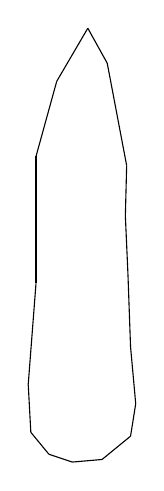
\begin{tikzpicture}
\draw (4.5033,8.8454) -- (4.7500,8.4013);
\draw (4.1086,8.1711) -- (4.5033,8.8454);
\draw (4.7500,8.4013) -- (4.9967,7.1020);
\draw (4.9803,6.4605) -- (4.9967,7.1020);
\draw (5.0461,4.7993) -- (5.0132,5.7204);
\draw (4.9803,6.4605) -- (5.0132,5.7204);
\draw (5.0461,4.7993) -- (5.1118,4.0757);
\draw (5.0461,3.6645) -- (4.6842,3.3684);
\draw (5.1118,4.0757) -- (5.0461,3.6645);
\draw (4.3059,3.3355) -- (4.0099,3.4342);
\draw (4.6842,3.3684) -- (4.3059,3.3355);
\draw (3.8454,5.6053) -- (3.8454,7.2171);
\draw (4.0099,3.4342) -- (3.7796,3.7138);
\draw (3.7796,3.7138) -- (3.7467,4.3224);
\draw (3.8454,5.6053) -- (3.7467,4.3224);
\draw (3.8454,7.2171) -- (4.1086,8.1711);
\fill (4.5033,8.8454) circle;
\fill (4.7500,8.4013) circle;
\fill (4.9967,7.1020) circle;
\fill (4.9803,6.4605) circle;
\fill (5.0132,5.7204) circle;
\fill (5.0461,4.7993) circle;
\fill (5.1118,4.0757) circle;
\fill (5.0461,3.6645) circle;
\fill (4.6842,3.3684) circle;
\fill (4.3059,3.3355) circle;
\fill (4.0099,3.4342) circle;
\fill (3.7796,3.7138) circle;
\fill (3.7467,4.3224) circle;
\fill (3.8454,5.6053) circle;
\fill (3.8454,7.2171) circle;
\fill (4.1086,8.1711) circle;
\end{tikzpicture}

\label{fig:exp:single_parameter_b:fifth}
\end{subfigure}%
\begin{subfigure}{.15\linewidth}
\centering
%% Include the picture as follows: \
% \begingroup
% \tikzset{every picture/.style={scale=1,radius=0.05,line width=0.4}}%
% \input{tikz/[filename].tex}%
% \endgroup
%
%% Want to add a label? Use node[<position>]{label},
%% where <position> is one of: below / above / left / right
% \fill (0,0) circle node[below]{$p_1$};
%% Want to give the point a different color?
% \fill[red] (0,0) circle;
%
\begin{tikzpicture}
\draw (1.7895,0.7270) -- (1.6908,1.8618);
\draw (2.7105,0.7105) -- (1.7895,0.7270);
\draw (1.6414,3.0625) -- (1.6908,1.8618);
\draw (1.5592,6.3191) -- (1.4934,5.5132);
\draw (1.6414,3.0625) -- (1.6086,4.1809);
\draw (1.5592,6.3191) -- (1.5921,7.3882);
\draw (2.6283,4.1480) -- (1.6086,4.1809);
\draw (2.6283,4.1480) -- (1.4934,5.5132);
\draw (2.6941,7.4539) -- (3.7303,7.0428);
\draw (1.5921,7.3882) -- (2.6941,7.4539);
\draw (3.8947,4.3289) -- (4.7007,5.0691);
\draw (4.5033,6.1875) -- (4.7007,5.0691);
\draw (3.7303,7.0428) -- (4.5033,6.1875);
\draw (3.3355,3.6875) -- (3.9605,3.0954);
\draw (3.3355,3.6875) -- (3.8947,4.3289);
\draw (3.6480,1.1711) -- (2.7105,0.7105);
\draw (3.9605,3.0954) -- (4.0921,2.0099);
\draw (4.0921,2.0099) -- (3.6480,1.1711);
\fill (1.7895,0.7270) circle;
\fill (1.6908,1.8618) circle;
\fill (1.6414,3.0625) circle;
\fill (1.6086,4.1809) circle;
\fill (1.4934,5.5132) circle;
\fill (1.5592,6.3191) circle;
\fill (1.5921,7.3882) circle;
\fill (2.6941,7.4539) circle;
\fill (3.7303,7.0428) circle;
\fill (4.5033,6.1875) circle;
\fill (4.7007,5.0691) circle;
\fill (3.8947,4.3289) circle;
\fill (2.6283,4.1480) circle;
\fill (3.3355,3.6875) circle;
\fill (3.9605,3.0954) circle;
\fill (4.0921,2.0099) circle;
\fill (3.6480,1.1711) circle;
\fill (2.7105,0.7105) circle;
\end{tikzpicture}

\label{fig:exp:single_parameter_b:sixth}
\centering
\end{subfigure}
\caption{The solutions for two inputs, using $k = 1.2$ (left), $k = 1.4$ (center) and $k = 1.6$ (right) (using squared segment lengths for the likelihood function)}
\end{figure}
\endgroup

\subsubsection{Multiple curves}
The accuracy of the multiple curve algorithm relies on the effectiveness of the initial solution. The description provided two ways to reach the initial solution. The original method is relatively expensive, so the alternative method was made available to make the algorithm feasible for bigger input sizes. In the next section, the experimental results of the initial solution are evaluated. Then, the transformation from the initial solution to the final solution is evaluated.

Since the initial solution is created by taking the shortest of all possible line segments, the algorithm works perfect for curves where the points are uniformly distributed over the lines of the desired figure.
In figure \ref{fig:exp:multiple_initial}, the two initial solutions are displayed for an input of points that resembles three closed curves. Although the points are not uniformly distributed, the initial solution \ref{fig:exp:multiple_initial:initial} is perfect, because the points of the individual curves are closer to each other than the points of the other curves.
The alternative initial solution \ref{fig:exp:multiple_initial:alternative} has four unconnected points. Each of the four points are far apart from each other, with the points in the center being among their nearest 10 neighbours. Since the alternative algorithm does not look past the 10 nearest neighbours, the other free points are not visible to the algorithm and therefore they remain disconnected.
The fact that these points are not connected is not necessarily bad. After all, one can argue that a snapshot of four points does not justify the creation of a sparse curve that is larger than the other curves that consist of many more points.

The alternative solution only selects a number of points in the neighbourhood of a point. When the number of neighbors is too small, many of the input points remain disconnected. The imperfect initial solution \ref{fig:exp:multiple_initial:alternative} can be resolved by doubling the number of neighbors, but the same problem would show up again if the density of the curves in the middle is doubled as well. Since this problem cannot be solved by increasing the number of neighbors, a practical number of neighbors is chosen.
Experiments show that using the 10 nearest neighbours is sufficient to get an accurate initial solution.

\begingroup
\tikzset{every picture/.style={scale=1,radius=0.05,line width=0.4}}%
\begin{figure}[ht!]
\centering
\begin{subfigure}{.33\linewidth}
\centering
%% Include the picture as follows: \
% \begingroup
% \tikzset{every picture/.style={scale=1,radius=0.05,line width=0.4}}%
% \input{tikz/[filename].tex}%
% \endgroup
%
%% Want to add a label? Use node[<position>]{label},
%% where <position> is one of: below / above / left / right
% \fill (0,0) circle node[below]{$p_1$};
%% Want to give the point a different color?
% \fill[red] (0,0) circle;
%
\begin{tikzpicture}
\fill (3.8947,8.3191) circle;
\fill (2.9737,7.4967) circle;
\fill (2.9737,6.7237) circle;
\fill (5.5559,7.0855) circle;
\fill (6.5428,9.0428) circle;
\fill (2.6118,9.1086) circle;
\fill (4.8980,5.9178) circle;
\fill (2.5132,5.4901) circle;
\fill (6.3783,5.3914) circle;
\fill (3.5164,6.2467) circle;
\fill (4.0263,6.0987) circle;
\fill (4.2401,6.0493) circle;
\fill (4.7664,8.2204) circle;
\fill (5.3586,7.7434) circle;
\fill (4.1250,7.4145) circle;
\fill (3.7796,7.2500) circle;
\fill (3.6316,6.9046) circle;
\fill (3.7796,6.7730) circle;
\fill (4.0263,6.5757) circle;
\fill (4.4704,6.4770) circle;
\fill (4.6349,7.2171) circle;
\fill (4.8322,7.0691) circle;
\fill (4.9803,6.8882) circle;
\fill (5.0461,6.6579) circle;
\fill (4.7829,6.4605) circle;
\fill (4.3882,7.3816) circle;
\end{tikzpicture}

\caption{Input}
\label{fig:exp:multiple_initial:input}
\end{subfigure}%
\begin{subfigure}{.33\linewidth}
\centering
%% Include the picture as follows: \
% \begingroup
% \tikzset{every picture/.style={scale=1,radius=0.05,line width=0.4}}%
% \input{tikz/[filename].tex}%
% \endgroup
%
%% Want to add a label? Use node[<position>]{label},
%% where <position> is one of: below / above / left / right
% \fill (0,0) circle node[below]{$p_1$};
%% Want to give the point a different color?
% \fill[red] (0,0) circle;
%
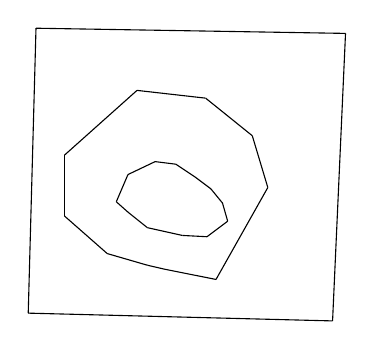
\begin{tikzpicture}
\draw (3.7796,7.2500) -- (3.6316,6.9046);
\draw (3.5164,6.2467) -- (4.0263,6.0987);
\draw (2.9737,6.7237) -- (3.5164,6.2467);
\draw (2.9737,7.4967) -- (2.9737,6.7237);
\draw (3.8947,8.3191) -- (2.9737,7.4967);
\draw (4.0263,6.0987) -- (4.2401,6.0493);
\draw (2.6118,9.1086) -- (2.5132,5.4901);
\draw (4.1250,7.4145) -- (3.7796,7.2500);
\draw (3.8947,8.3191) -- (4.7664,8.2204);
\draw (3.6316,6.9046) -- (3.7796,6.7730);
\draw (4.8980,5.9178) -- (4.2401,6.0493);
\draw (5.0461,6.6579) -- (4.7829,6.4605);
\draw (3.7796,6.7730) -- (4.0263,6.5757);
\draw (2.5132,5.4901) -- (6.3783,5.3914);
\draw (4.7664,8.2204) -- (5.3586,7.7434);
\draw (4.6349,7.2171) -- (4.8322,7.0691);
\draw (4.8322,7.0691) -- (4.9803,6.8882);
\draw (4.6349,7.2171) -- (4.3882,7.3816);
\draw (6.5428,9.0428) -- (2.6118,9.1086);
\draw (5.5559,7.0855) -- (4.8980,5.9178);
\draw (6.5428,9.0428) -- (6.3783,5.3914);
\draw (4.1250,7.4145) -- (4.3882,7.3816);
\draw (4.9803,6.8882) -- (5.0461,6.6579);
\draw (5.5559,7.0855) -- (5.3586,7.7434);
\draw (4.4704,6.4770) -- (4.7829,6.4605);
\draw (4.0263,6.5757) -- (4.4704,6.4770);
\fill (3.8947,8.3191) circle;
\fill (2.9737,7.4967) circle;
\fill (2.9737,6.7237) circle;
\fill (5.5559,7.0855) circle;
\fill (6.5428,9.0428) circle;
\fill (2.6118,9.1086) circle;
\fill (4.8980,5.9178) circle;
\fill (2.5132,5.4901) circle;
\fill (6.3783,5.3914) circle;
\fill (3.5164,6.2467) circle;
\fill (4.0263,6.0987) circle;
\fill (4.2401,6.0493) circle;
\fill (4.7664,8.2204) circle;
\fill (5.3586,7.7434) circle;
\fill (4.1250,7.4145) circle;
\fill (3.7796,7.2500) circle;
\fill (3.6316,6.9046) circle;
\fill (3.7796,6.7730) circle;
\fill (4.0263,6.5757) circle;
\fill (4.4704,6.4770) circle;
\fill (4.6349,7.2171) circle;
\fill (4.8322,7.0691) circle;
\fill (4.9803,6.8882) circle;
\fill (5.0461,6.6579) circle;
\fill (4.7829,6.4605) circle;
\fill (4.3882,7.3816) circle;
\end{tikzpicture}

\caption{Initial solution}
\label{fig:exp:multiple_initial:initial}
\end{subfigure}%
\begin{subfigure}{.33\linewidth}
\centering
%% Include the picture as follows: \
% \begingroup
% \tikzset{every picture/.style={scale=1,radius=0.05,line width=0.4}}%
% \input{tikz/[filename].tex}%
% \endgroup
%
%% Want to add a label? Use node[<position>]{label},
%% where <position> is one of: below / above / left / right
% \fill (0,0) circle node[below]{$p_1$};
%% Want to give the point a different color?
% \fill[red] (0,0) circle;
%
\begin{tikzpicture}
\draw (3.7796,7.2500) -- (3.6316,6.9046);
\draw (3.7796,6.7730) -- (4.0263,6.5757);
\draw (3.5164,6.2467) -- (4.0263,6.0987);
\draw (2.9737,6.7237) -- (3.5164,6.2467);
\draw (2.9737,7.4967) -- (2.9737,6.7237);
\draw (3.8947,8.3191) -- (2.9737,7.4967);
\draw (4.7664,8.2204) -- (5.3586,7.7434);
\draw (4.6349,7.2171) -- (4.8322,7.0691);
\draw (4.0263,6.0987) -- (4.2401,6.0493);
\draw (4.8322,7.0691) -- (4.9803,6.8882);
\draw (4.1250,7.4145) -- (3.7796,7.2500);
\draw (4.6349,7.2171) -- (4.3882,7.3816);
\draw (5.5559,7.0855) -- (4.8980,5.9178);
\draw (3.8947,8.3191) -- (4.7664,8.2204);
\draw (3.6316,6.9046) -- (3.7796,6.7730);
\draw (4.1250,7.4145) -- (4.3882,7.3816);
\draw (4.8980,5.9178) -- (4.2401,6.0493);
\draw (5.5559,7.0855) -- (5.3586,7.7434);
\draw (4.9803,6.8882) -- (5.0461,6.6579);
\draw (4.4704,6.4770) -- (4.7829,6.4605);
\draw (4.0263,6.5757) -- (4.4704,6.4770);
\draw (5.0461,6.6579) -- (4.7829,6.4605);
\fill (3.8947,8.3191) circle;
\fill (2.9737,7.4967) circle;
\fill (2.9737,6.7237) circle;
\fill (5.5559,7.0855) circle;
\fill (6.5428,9.0428) circle;
\fill (2.6118,9.1086) circle;
\fill (4.8980,5.9178) circle;
\fill (2.5132,5.4901) circle;
\fill (6.3783,5.3914) circle;
\fill (3.5164,6.2467) circle;
\fill (4.0263,6.0987) circle;
\fill (4.2401,6.0493) circle;
\fill (4.7664,8.2204) circle;
\fill (5.3586,7.7434) circle;
\fill (4.1250,7.4145) circle;
\fill (3.7796,7.2500) circle;
\fill (3.6316,6.9046) circle;
\fill (3.7796,6.7730) circle;
\fill (4.0263,6.5757) circle;
\fill (4.4704,6.4770) circle;
\fill (4.6349,7.2171) circle;
\fill (4.8322,7.0691) circle;
\fill (4.9803,6.8882) circle;
\fill (5.0461,6.6579) circle;
\fill (4.7829,6.4605) circle;
\fill (4.3882,7.3816) circle;
\end{tikzpicture}

\caption{Alternative initial solution}
\label{fig:exp:multiple_initial:alternative}
\end{subfigure}
\caption{The initial solutions for three curves}
\label{fig:exp:multiple_initial}
\end{figure}
\endgroup

Figure \ref{fig:exp:multiple_split_triangles:initial} shows an initial solution that consists of 4 curves. The solution looks reasonable, but note that three of these curves are triangles with a very sharp corner. This is a very typical initial solution, caused by the fact that only lengths of the segments are used in the first step of the algorithm. After connecting the three points at the bottom of picture \ref{fig:exp:multiple_split_triangles:initial:input}, all of the three points have degree two and will no longer accept connections with other points, even though two of these points are very close to the left and right points (which also form a triangle, ultimately).

This problem of generating triangles is very common, and sufficiently solved by the second step of the algorithm, as seen in figure \ref{fig:exp:multiple_split_triangles:output}. All triangles have been identified and merged into one big curve. Not entirely coincidentally, this example shows that the removed segments are the longest segments within the triangle. This happens quite often, because the triangle problem is caused by abusively connecting one endpoint of a short curve with the other endpoint of the same short curve.

\begingroup
\tikzset{every picture/.style={scale=1,radius=0.05,line width=0.4}}%
\begin{figure}[ht!]
\centering
\begin{subfigure}{.33\linewidth}
\centering
%% Include the picture as follows: \
% \begingroup
% \tikzset{every picture/.style={scale=1,radius=0.05,line width=0.4}}%
% \input{tikz/[filename].tex}%
% \endgroup
%
%% Want to add a label? Use node[<position>]{label},
%% where <position> is one of: below / above / left / right
% \fill (0,0) circle node[below]{$p_1$};
%% Want to give the point a different color?
% \fill[red] (0,0) circle;
%
\begin{tikzpicture}
\fill (3.7796,7.1184) circle;
\fill (4.1414,7.2500) circle;
\fill (5.0789,7.4474) circle;
\fill (5.7204,7.4803) circle;
\fill (6.5921,7.2500) circle;
\fill (3.9276,6.4770) circle;
\fill (4.4046,5.5395) circle;
\fill (5.4079,5.0789) circle;
\fill (6.4276,5.4079) circle;
\fill (5.2928,6.6086) circle;
\fill (5.2105,6.4112) circle;
\fill (5.3750,6.3289) circle;
\fill (5.4901,6.4112) circle;
\end{tikzpicture}

\caption{Input}
\label{fig:exp:multiple_split_triangles:initial:input}
\end{subfigure}%
\begin{subfigure}{.33\linewidth}
\centering
%% Include the picture as follows: \
% \begingroup
% \tikzset{every picture/.style={scale=1,radius=0.05,line width=0.4}}%
% \input{tikz/[filename].tex}%
% \endgroup
%
%% Want to add a label? Use node[<position>]{label},
%% where <position> is one of: below / above / left / right
% \fill (0,0) circle node[below]{$p_1$};
%% Want to give the point a different color?
% \fill[red] (0,0) circle;
%
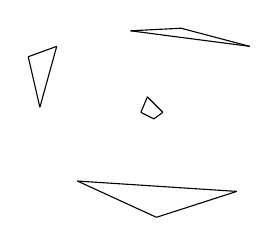
\begin{tikzpicture}
\draw (3.7796,7.1184) -- (4.1414,7.2500);
\draw (5.4079,5.0789) -- (6.4276,5.4079);
\draw (5.0789,7.4474) -- (6.5921,7.2500);
\draw (5.0789,7.4474) -- (5.7204,7.4803);
\draw (3.7796,7.1184) -- (3.9276,6.4770);
\draw (5.2105,6.4112) -- (5.3750,6.3289);
\draw (4.1414,7.2500) -- (3.9276,6.4770);
\draw (5.7204,7.4803) -- (6.5921,7.2500);
\draw (4.4046,5.5395) -- (6.4276,5.4079);
\draw (5.3750,6.3289) -- (5.4901,6.4112);
\draw (4.4046,5.5395) -- (5.4079,5.0789);
\draw (5.2928,6.6086) -- (5.2105,6.4112);
\draw (5.2928,6.6086) -- (5.4901,6.4112);
\fill (3.7796,7.1184) circle;
\fill (4.1414,7.2500) circle;
\fill (5.0789,7.4474) circle;
\fill (5.7204,7.4803) circle;
\fill (6.5921,7.2500) circle;
\fill (3.9276,6.4770) circle;
\fill (4.4046,5.5395) circle;
\fill (5.4079,5.0789) circle;
\fill (6.4276,5.4079) circle;
\fill (5.2928,6.6086) circle;
\fill (5.2105,6.4112) circle;
\fill (5.3750,6.3289) circle;
\fill (5.4901,6.4112) circle;
\end{tikzpicture}

\caption{Initial solution}
\label{fig:exp:multiple_split_triangles:initial}
\end{subfigure}%
\begin{subfigure}{.33\linewidth}
\centering
%% Include the picture as follows: \
% \begingroup
% \tikzset{every picture/.style={scale=1,radius=0.05,line width=0.4}}%
% \input{tikz/[filename].tex}%
% \endgroup
%
%% Want to add a label? Use node[<position>]{label},
%% where <position> is one of: below / above / left / right
% \fill (0,0) circle node[below]{$p_1$};
%% Want to give the point a different color?
% \fill[red] (0,0) circle;
%
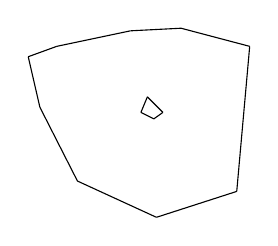
\begin{tikzpicture}
\draw (3.7796,7.1184) -- (4.1414,7.2500);
\draw (5.4079,5.0789) -- (6.4276,5.4079);
\draw (5.0789,7.4474) -- (5.7204,7.4803);
\draw (3.7796,7.1184) -- (3.9276,6.4770);
\draw (5.2105,6.4112) -- (5.3750,6.3289);
\draw (5.7204,7.4803) -- (6.5921,7.2500);
\draw (5.3750,6.3289) -- (5.4901,6.4112);
\draw (4.4046,5.5395) -- (5.4079,5.0789);
\draw (4.1414,7.2500) -- (5.0789,7.4474);
\draw (3.9276,6.4770) -- (4.4046,5.5395);
\draw (6.5921,7.2500) -- (6.4276,5.4079);
\draw (5.2928,6.6086) -- (5.2105,6.4112);
\draw (5.2928,6.6086) -- (5.4901,6.4112);
\fill (3.7796,7.1184) circle;
\fill (4.1414,7.2500) circle;
\fill (5.0789,7.4474) circle;
\fill (5.7204,7.4803) circle;
\fill (6.5921,7.2500) circle;
\fill (3.9276,6.4770) circle;
\fill (4.4046,5.5395) circle;
\fill (5.4079,5.0789) circle;
\fill (6.4276,5.4079) circle;
\fill (5.2928,6.6086) circle;
\fill (5.2105,6.4112) circle;
\fill (5.3750,6.3289) circle;
\fill (5.4901,6.4112) circle;
\end{tikzpicture}

\caption{Final solution}
\label{fig:exp:multiple_split_triangles:output}
\end{subfigure}
\caption{The final solution consisting of two curves derived via the initial solution}
\label{fig:exp:multiple_split_triangles}
\end{figure}
\endgroup

$\alpha_{required}$ and $\alpha_{sharp}$ are designed to reduce the (non-asymptotic) running time of the algorithm.\\
When $\alpha_{required}$ is set to $0\degree$, then segments are never replaced because all angles are considered to be fine. Hence it does not make sense to pick a low value for $\alpha_{required}$. Setting the value to the other extreme value, $180\degree$, does not make sense either, because the number of unnecessary calculations increase. Choosing $\alpha_{required} = 90\degree$ did not have a negative effect on the final result. This makes sense, because the second step of the algorithm is designed to cope with the triangle problem, and the angles of the sharp corners in a triangle never exceed $90\degree$.\\
When $\alpha_{sharp}$ is set to $180\degree$, then the angles with alternative segments are considered to be too sharp, hence none of the segments will be replaced. If it is set to $0\degree$, then none of the segments will be excluded, and the algorithm evaluates for each of the $10$ neighbors of every sharp corner whether it makes sense to replace an existing segment with a new segment to the neighbor.

These parameters were designed to speed up the algorithm, but no evidence for such speed improvements were found during tests with 1000 and 10000 points. This might be caused by the fact that the majority of the alternative segments are ruled out during the initial steps of the "best point" finding algorithm that runs in constant time.

When the distance between a point and another point is more than $\textsc{DistanceMultiplier}$, then the line segment between these two points will never be considered as a suitable replacement. Figure \ref{fig:exp:multiple_length_factor:1} shows that two triangles are not connected due to a $\textsc{DistanceMultiplier}$ factor of 1. After increasing this parameter value to $1.2$, the triangles are joined into one curve. $1.2$ turns out to be the ideal value for this parameter. When the parameter is incremented to $1.5$, then some curves are mistakenly joined, as seen as figure \ref{fig:exp:multiple_face}.

\begingroup
\tikzset{every picture/.style={scale=0.5,radius=0.10,line width=0.4,rotate=70}}%
\begin{figure}[ht!]
\centering
\begin{subfigure}{.33\linewidth}
\centering
%% Include the picture as follows: \
% \begingroup
% \tikzset{every picture/.style={scale=1,radius=0.05,line width=0.4}}%
% \input{tikz/[filename].tex}%
% \endgroup
%
%% Want to add a label? Use node[<position>]{label},
%% where <position> is one of: below / above / left / right
% \fill (0,0) circle node[below]{$p_1$};
%% Want to give the point a different color?
% \fill[red] (0,0) circle;
%
\begin{tikzpicture}
\fill (3.0724,1.3783) circle;
\fill (6.2467,1.2303) circle;
\fill (3.3849,5.1776) circle;
\fill (6.7895,4.9967) circle;
\fill (4.6349,0.5395) circle;
\fill (5.4572,9.8651) circle;
\end{tikzpicture}

\caption{Input}
\label{fig:exp:multiple_length_factor:input}
\end{subfigure}%
\begin{subfigure}{.33\linewidth}
\centering
%% Include the picture as follows: \
% \begingroup
% \tikzset{every picture/.style={scale=1,radius=0.05,line width=0.4}}%
% \input{tikz/[filename].tex}%
% \endgroup
%
%% Want to add a label? Use node[<position>]{label},
%% where <position> is one of: below / above / left / right
% \fill (0,0) circle node[below]{$p_1$};
%% Want to give the point a different color?
% \fill[red] (0,0) circle;
%
\begin{tikzpicture}
\draw (6.7895,4.9967) -- (5.4572,9.8651);
\draw (3.0724,1.3783) -- (6.2467,1.2303);
\draw (3.0724,1.3783) -- (4.6349,0.5395);
\draw (6.2467,1.2303) -- (4.6349,0.5395);
\draw (3.3849,5.1776) -- (5.4572,9.8651);
\draw (3.3849,5.1776) -- (6.7895,4.9967);
\fill (3.0724,1.3783) circle;
\fill (6.2467,1.2303) circle;
\fill (3.3849,5.1776) circle;
\fill (6.7895,4.9967) circle;
\fill (4.6349,0.5395) circle;
\fill (5.4572,9.8651) circle;
\end{tikzpicture}

\caption{$\textsc{DistanceMultiplier} = 1$}
\label{fig:exp:multiple_length_factor:1}
\end{subfigure}%
\begin{subfigure}{.33\linewidth}
\centering
%% Include the picture as follows: \
% \begingroup
% \tikzset{every picture/.style={scale=1,radius=0.05,line width=0.4}}%
% \input{tikz/[filename].tex}%
% \endgroup
%
%% Want to add a label? Use node[<position>]{label},
%% where <position> is one of: below / above / left / right
% \fill (0,0) circle node[below]{$p_1$};
%% Want to give the point a different color?
% \fill[red] (0,0) circle;
%
\begin{tikzpicture}
\draw (6.7895,4.9967) -- (5.4572,9.8651);
\draw (3.0724,1.3783) -- (3.3849,5.1776);
\draw (3.0724,1.3783) -- (4.6349,0.5395);
\draw (6.2467,1.2303) -- (6.7895,4.9967);
\draw (6.2467,1.2303) -- (4.6349,0.5395);
\draw (3.3849,5.1776) -- (5.4572,9.8651);
\fill (3.0724,1.3783) circle;
\fill (6.2467,1.2303) circle;
\fill (3.3849,5.1776) circle;
\fill (6.7895,4.9967) circle;
\fill (4.6349,0.5395) circle;
\fill (5.4572,9.8651) circle;
\end{tikzpicture}

\caption{$\textsc{DistanceMultiplier} = 1.2$}
\label{fig:exp:multiple_length_factor:1.2}
\end{subfigure}
\caption{Output for different values of $\textsc{DistanceMultiplier}$}
\label{fig:exp:multiple_length_factor}
\end{figure}
\endgroup
\begingroup
\tikzset{every picture/.style={scale=0.5,radius=0.10,line width=0.5}}%
\begin{figure}[ht!]
\centering
\begin{subfigure}{.33\linewidth}
\centering
%% Include the picture as follows: \
% \begingroup
% \tikzset{every picture/.style={scale=1,radius=0.05,line width=0.4}}%
% \input{tikz/[filename].tex}%
% \endgroup
%
%% Want to add a label? Use node[<position>]{label},
%% where <position> is one of: below / above / left / right
% \fill (0,0) circle node[below]{$p_1$};
%% Want to give the point a different color?
% \fill[red] (0,0) circle;
%
\begin{tikzpicture}
\fill (2.2664,8.6151) circle;
\fill (1.7401,8.0395) circle;
\fill (1.3947,6.7895) circle;
\fill (1.3454,5.4737) circle;
\fill (1.4441,4.8816) circle;
\fill (1.7401,3.6974) circle;
\fill (2.4474,2.7928) circle;
\fill (3.6316,2.2664) circle;
\fill (4.9967,2.2171) circle;
\fill (6.1974,3.1217) circle;
\fill (6.6414,4.3882) circle;
\fill (6.9375,5.9178) circle;
\fill (6.7237,7.2664) circle;
\fill (6.1151,8.3849) circle;
\fill (5.3257,8.8783) circle;
\fill (4.2237,9.0428) circle;
\fill (3.0230,8.8783) circle;
\fill (3.0066,4.2566) circle;
\fill (3.3191,3.8783) circle;
\fill (3.7303,3.7467) circle;
\fill (4.1743,3.6480) circle;
\fill (4.5526,3.6974) circle;
\fill (5.0461,4.1579) circle;
\fill (4.5362,4.3224) circle;
\fill (3.8947,4.3388) circle;
\fill (3.4013,4.3882) circle;
\fill (4.1414,6.3125) circle;
\fill (3.8125,5.6053) circle;
\fill (4.3059,5.5395) circle;
\fill (3.0559,7.7599) circle;
\fill (2.7599,7.3816) circle;
\fill (2.7270,7.0526) circle;
\fill (3.0888,6.9046) circle;
\fill (3.6809,6.8882) circle;
\fill (3.8289,7.2171) circle;
\fill (3.5164,7.5296) circle;
\fill (4.7007,6.7072) circle;
\fill (5.2434,6.6250) circle;
\fill (5.7862,6.7237) circle;
\fill (5.8849,7.0033) circle;
\fill (5.7204,7.4967) circle;
\fill (5.2434,7.4967) circle;
\fill (4.7993,7.1020) circle;
\fill (4.8487,3.9342) circle;
\fill (4.2566,4.3618) circle;
\fill (4.2566,6.0395) circle;
\fill (4.2895,5.8092) circle;
\fill (3.9112,5.8421) circle;
\fill (3.9605,6.0888) circle;
\fill (4.0757,5.5461) circle;
\end{tikzpicture}

\caption{Input}
\label{fig:exp:multiple_face:input}
\end{subfigure}%
\begin{subfigure}{.33\linewidth}
\centering
%% Include the picture as follows: \
% \begingroup
% \tikzset{every picture/.style={scale=1,radius=0.05,line width=0.4}}%
% \input{tikz/[filename].tex}%
% \endgroup
%
%% Want to add a label? Use node[<position>]{label},
%% where <position> is one of: below / above / left / right
% \fill (0,0) circle node[below]{$p_1$};
%% Want to give the point a different color?
% \fill[red] (0,0) circle;
%
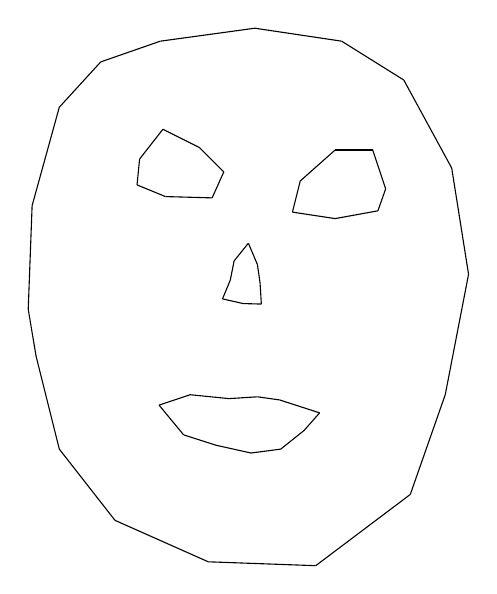
\begin{tikzpicture}
\draw (1.7401,3.6974) -- (2.4474,2.7928);
\draw (3.6809,6.8882) -- (3.8289,7.2171);
\draw (6.1974,3.1217) -- (6.6414,4.3882);
\draw (6.7237,7.2664) -- (6.1151,8.3849);
\draw (6.9375,5.9178) -- (6.7237,7.2664);
\draw (4.9967,2.2171) -- (6.1974,3.1217);
\draw (4.5362,4.3224) -- (4.2566,4.3618);
\draw (3.0066,4.2566) -- (3.4013,4.3882);
\draw (3.0066,4.2566) -- (3.3191,3.8783);
\draw (3.3191,3.8783) -- (3.7303,3.7467);
\draw (5.7204,7.4967) -- (5.2434,7.4967);
\draw (5.3257,8.8783) -- (4.2237,9.0428);
\draw (3.8289,7.2171) -- (3.5164,7.5296);
\draw (2.7599,7.3816) -- (2.7270,7.0526);
\draw (3.6316,2.2664) -- (4.9967,2.2171);
\draw (3.0559,7.7599) -- (3.5164,7.5296);
\draw (3.0559,7.7599) -- (2.7599,7.3816);
\draw (6.1151,8.3849) -- (5.3257,8.8783);
\draw (4.1743,3.6480) -- (4.5526,3.6974);
\draw (4.2566,6.0395) -- (4.2895,5.8092);
\draw (1.3947,6.7895) -- (1.3454,5.4737);
\draw (4.2237,9.0428) -- (3.0230,8.8783);
\draw (4.7007,6.7072) -- (5.2434,6.6250);
\draw (3.8125,5.6053) -- (3.9112,5.8421);
\draw (5.0461,4.1579) -- (4.8487,3.9342);
\draw (3.8125,5.6053) -- (4.0757,5.5461);
\draw (3.9112,5.8421) -- (3.9605,6.0888);
\draw (1.7401,8.0395) -- (1.3947,6.7895);
\draw (4.7007,6.7072) -- (4.7993,7.1020);
\draw (5.2434,6.6250) -- (5.7862,6.7237);
\draw (4.3059,5.5395) -- (4.0757,5.5461);
\draw (4.3059,5.5395) -- (4.2895,5.8092);
\draw (5.0461,4.1579) -- (4.5362,4.3224);
\draw (1.4441,4.8816) -- (1.7401,3.6974);
\draw (6.6414,4.3882) -- (6.9375,5.9178);
\draw (1.3454,5.4737) -- (1.4441,4.8816);
\draw (2.7270,7.0526) -- (3.0888,6.9046);
\draw (3.8947,4.3388) -- (4.2566,4.3618);
\draw (2.2664,8.6151) -- (3.0230,8.8783);
\draw (5.8849,7.0033) -- (5.7204,7.4967);
\draw (5.7862,6.7237) -- (5.8849,7.0033);
\draw (3.8947,4.3388) -- (3.4013,4.3882);
\draw (4.5526,3.6974) -- (4.8487,3.9342);
\draw (4.1414,6.3125) -- (4.2566,6.0395);
\draw (2.4474,2.7928) -- (3.6316,2.2664);
\draw (3.7303,3.7467) -- (4.1743,3.6480);
\draw (4.1414,6.3125) -- (3.9605,6.0888);
\draw (3.0888,6.9046) -- (3.6809,6.8882);
\draw (5.2434,7.4967) -- (4.7993,7.1020);
\draw (2.2664,8.6151) -- (1.7401,8.0395);
\fill (2.2664,8.6151) circle;
\fill (1.7401,8.0395) circle;
\fill (1.3947,6.7895) circle;
\fill (1.3454,5.4737) circle;
\fill (1.4441,4.8816) circle;
\fill (1.7401,3.6974) circle;
\fill (2.4474,2.7928) circle;
\fill (3.6316,2.2664) circle;
\fill (4.9967,2.2171) circle;
\fill (6.1974,3.1217) circle;
\fill (6.6414,4.3882) circle;
\fill (6.9375,5.9178) circle;
\fill (6.7237,7.2664) circle;
\fill (6.1151,8.3849) circle;
\fill (5.3257,8.8783) circle;
\fill (4.2237,9.0428) circle;
\fill (3.0230,8.8783) circle;
\fill (3.0066,4.2566) circle;
\fill (3.3191,3.8783) circle;
\fill (3.7303,3.7467) circle;
\fill (4.1743,3.6480) circle;
\fill (4.5526,3.6974) circle;
\fill (5.0461,4.1579) circle;
\fill (4.5362,4.3224) circle;
\fill (3.8947,4.3388) circle;
\fill (3.4013,4.3882) circle;
\fill (4.1414,6.3125) circle;
\fill (3.8125,5.6053) circle;
\fill (4.3059,5.5395) circle;
\fill (3.0559,7.7599) circle;
\fill (2.7599,7.3816) circle;
\fill (2.7270,7.0526) circle;
\fill (3.0888,6.9046) circle;
\fill (3.6809,6.8882) circle;
\fill (3.8289,7.2171) circle;
\fill (3.5164,7.5296) circle;
\fill (4.7007,6.7072) circle;
\fill (5.2434,6.6250) circle;
\fill (5.7862,6.7237) circle;
\fill (5.8849,7.0033) circle;
\fill (5.7204,7.4967) circle;
\fill (5.2434,7.4967) circle;
\fill (4.7993,7.1020) circle;
\fill (4.8487,3.9342) circle;
\fill (4.2566,4.3618) circle;
\fill (4.2566,6.0395) circle;
\fill (4.2895,5.8092) circle;
\fill (3.9112,5.8421) circle;
\fill (3.9605,6.0888) circle;
\fill (4.0757,5.5461) circle;
\end{tikzpicture}

\caption{$\textsc{DistanceMultiplier} = 1.2$}
\label{fig:exp:multiple_face:1.2}
\end{subfigure}%
\begin{subfigure}{.33\linewidth}
\centering
%% Include the picture as follows: \
% \begingroup
% \tikzset{every picture/.style={scale=1,radius=0.05,line width=0.4}}%
% \input{tikz/[filename].tex}%
% \endgroup
%
%% Want to add a label? Use node[<position>]{label},
%% where <position> is one of: below / above / left / right
% \fill (0,0) circle node[below]{$p_1$};
%% Want to give the point a different color?
% \fill[red] (0,0) circle;
%
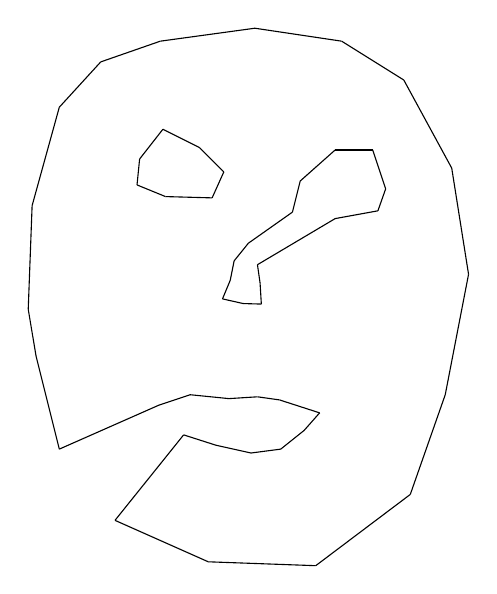
\begin{tikzpicture}
\draw (3.6809,6.8882) -- (3.8289,7.2171);
\draw (6.1974,3.1217) -- (6.6414,4.3882);
\draw (6.7237,7.2664) -- (6.1151,8.3849);
\draw (6.9375,5.9178) -- (6.7237,7.2664);
\draw (4.9967,2.2171) -- (6.1974,3.1217);
\draw (3.3191,3.8783) -- (2.4474,2.7928);
\draw (4.5362,4.3224) -- (4.2566,4.3618);
\draw (3.0066,4.2566) -- (3.4013,4.3882);
\draw (3.3191,3.8783) -- (3.7303,3.7467);
\draw (5.7204,7.4967) -- (5.2434,7.4967);
\draw (5.3257,8.8783) -- (4.2237,9.0428);
\draw (3.8289,7.2171) -- (3.5164,7.5296);
\draw (2.7599,7.3816) -- (2.7270,7.0526);
\draw (3.6316,2.2664) -- (4.9967,2.2171);
\draw (3.0559,7.7599) -- (3.5164,7.5296);
\draw (3.0559,7.7599) -- (2.7599,7.3816);
\draw (6.1151,8.3849) -- (5.3257,8.8783);
\draw (4.2566,6.0395) -- (5.2434,6.6250);
\draw (4.1743,3.6480) -- (4.5526,3.6974);
\draw (4.2566,6.0395) -- (4.2895,5.8092);
\draw (1.3947,6.7895) -- (1.3454,5.4737);
\draw (4.2237,9.0428) -- (3.0230,8.8783);
\draw (3.8125,5.6053) -- (3.9112,5.8421);
\draw (5.0461,4.1579) -- (4.8487,3.9342);
\draw (3.8125,5.6053) -- (4.0757,5.5461);
\draw (3.9112,5.8421) -- (3.9605,6.0888);
\draw (1.7401,8.0395) -- (1.3947,6.7895);
\draw (4.7007,6.7072) -- (4.7993,7.1020);
\draw (5.2434,6.6250) -- (5.7862,6.7237);
\draw (4.3059,5.5395) -- (4.0757,5.5461);
\draw (4.3059,5.5395) -- (4.2895,5.8092);
\draw (5.0461,4.1579) -- (4.5362,4.3224);
\draw (1.4441,4.8816) -- (1.7401,3.6974);
\draw (6.6414,4.3882) -- (6.9375,5.9178);
\draw (1.3454,5.4737) -- (1.4441,4.8816);
\draw (2.7270,7.0526) -- (3.0888,6.9046);
\draw (3.8947,4.3388) -- (4.2566,4.3618);
\draw (2.2664,8.6151) -- (3.0230,8.8783);
\draw (5.8849,7.0033) -- (5.7204,7.4967);
\draw (5.7862,6.7237) -- (5.8849,7.0033);
\draw (3.8947,4.3388) -- (3.4013,4.3882);
\draw (4.5526,3.6974) -- (4.8487,3.9342);
\draw (3.0066,4.2566) -- (1.7401,3.6974);
\draw (2.4474,2.7928) -- (3.6316,2.2664);
\draw (3.7303,3.7467) -- (4.1743,3.6480);
\draw (4.1414,6.3125) -- (3.9605,6.0888);
\draw (3.0888,6.9046) -- (3.6809,6.8882);
\draw (4.1414,6.3125) -- (4.7007,6.7072);
\draw (5.2434,7.4967) -- (4.7993,7.1020);
\draw (2.2664,8.6151) -- (1.7401,8.0395);
\fill (2.2664,8.6151) circle;
\fill (1.7401,8.0395) circle;
\fill (1.3947,6.7895) circle;
\fill (1.3454,5.4737) circle;
\fill (1.4441,4.8816) circle;
\fill (1.7401,3.6974) circle;
\fill (2.4474,2.7928) circle;
\fill (3.6316,2.2664) circle;
\fill (4.9967,2.2171) circle;
\fill (6.1974,3.1217) circle;
\fill (6.6414,4.3882) circle;
\fill (6.9375,5.9178) circle;
\fill (6.7237,7.2664) circle;
\fill (6.1151,8.3849) circle;
\fill (5.3257,8.8783) circle;
\fill (4.2237,9.0428) circle;
\fill (3.0230,8.8783) circle;
\fill (3.0066,4.2566) circle;
\fill (3.3191,3.8783) circle;
\fill (3.7303,3.7467) circle;
\fill (4.1743,3.6480) circle;
\fill (4.5526,3.6974) circle;
\fill (5.0461,4.1579) circle;
\fill (4.5362,4.3224) circle;
\fill (3.8947,4.3388) circle;
\fill (3.4013,4.3882) circle;
\fill (4.1414,6.3125) circle;
\fill (3.8125,5.6053) circle;
\fill (4.3059,5.5395) circle;
\fill (3.0559,7.7599) circle;
\fill (2.7599,7.3816) circle;
\fill (2.7270,7.0526) circle;
\fill (3.0888,6.9046) circle;
\fill (3.6809,6.8882) circle;
\fill (3.8289,7.2171) circle;
\fill (3.5164,7.5296) circle;
\fill (4.7007,6.7072) circle;
\fill (5.2434,6.6250) circle;
\fill (5.7862,6.7237) circle;
\fill (5.8849,7.0033) circle;
\fill (5.7204,7.4967) circle;
\fill (5.2434,7.4967) circle;
\fill (4.7993,7.1020) circle;
\fill (4.8487,3.9342) circle;
\fill (4.2566,4.3618) circle;
\fill (4.2566,6.0395) circle;
\fill (4.2895,5.8092) circle;
\fill (3.9112,5.8421) circle;
\fill (3.9605,6.0888) circle;
\fill (4.0757,5.5461) circle;
\end{tikzpicture}

\caption{$\textsc{DistanceMultiplier} = 1.5$}
\label{fig:exp:multiple_face:1.5}
\end{subfigure}
\caption{Varying $\textsc{DistanceMultiplier}$ for a set of points that resembles a face}
\label{fig:exp:multiple_face}
\end{figure}
\endgroup

Figure \ref{fig:exp:multiple_weight} shows the outputs for $\textsc{minWeight} = -0.2$ and $2$. As predicted in the description of the algorithm, none of the segments from the initial solution are replaced when the parameter is set to $2$.
\begingroup
\tikzset{every picture/.style={scale=1,radius=0.05,line width=0.4}}%
\begin{figure}[ht!]
\centering
\begin{subfigure}{.25\linewidth}
\centering
%% Include the picture as follows: \
% \begingroup
% \tikzset{every picture/.style={scale=1,radius=0.05,line width=0.4}}%
% \input{tikz/[filename].tex}%
% \endgroup
%
%% Want to add a label? Use node[<position>]{label},
%% where <position> is one of: below / above / left / right
% \fill (0,0) circle node[below]{$p_1$};
%% Want to give the point a different color?
% \fill[red] (0,0) circle;
%
\begin{tikzpicture}
\fill (4.4211,3.9671) circle;
\fill (4.5691,4.0164) circle;
\fill (4.9967,4.0000) circle;
\fill (5.0789,3.9507) circle;
\fill (4.9638,3.6711) circle;
\fill (4.7829,3.4572) circle;
\fill (4.7007,3.4408) circle;
\fill (4.4704,3.6711) circle;
\fill (4.4046,3.9178) circle;
\fill (4.8322,4.1151) circle;
\fill (4.8816,4.1151) circle;
\fill (4.7664,4.0329) circle;
\end{tikzpicture}

\caption{Input}
\label{fig:exp:multiple_weight:input}
\end{subfigure}%
\begin{subfigure}{.25\linewidth}
\centering
%% Include the picture as follows: \
% \begingroup
% \tikzset{every picture/.style={scale=1,radius=0.05,line width=0.4}}%
% \input{tikz/[filename].tex}%
% \endgroup
%
%% Want to add a label? Use node[<position>]{label},
%% where <position> is one of: below / above / left / right
% \fill (0,0) circle node[below]{$p_1$};
%% Want to give the point a different color?
% \fill[red] (0,0) circle;
%
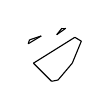
\begin{tikzpicture}
\draw (4.7829,3.4572) -- (4.7007,3.4408);
\draw (4.9967,4.0000) -- (4.4704,3.6711);
\draw (4.4211,3.9671) -- (4.5691,4.0164);
\draw (4.9638,3.6711) -- (4.7829,3.4572);
\draw (4.5691,4.0164) -- (4.4046,3.9178);
\draw (4.7007,3.4408) -- (4.4704,3.6711);
\draw (4.8816,4.1151) -- (4.7664,4.0329);
\draw (4.8322,4.1151) -- (4.8816,4.1151);
\draw (4.4211,3.9671) -- (4.4046,3.9178);
\draw (5.0789,3.9507) -- (4.9638,3.6711);
\draw (4.8322,4.1151) -- (4.7664,4.0329);
\draw (4.9967,4.0000) -- (5.0789,3.9507);
\fill (4.4211,3.9671) circle;
\fill (4.5691,4.0164) circle;
\fill (4.9967,4.0000) circle;
\fill (5.0789,3.9507) circle;
\fill (4.9638,3.6711) circle;
\fill (4.7829,3.4572) circle;
\fill (4.7007,3.4408) circle;
\fill (4.4704,3.6711) circle;
\fill (4.4046,3.9178) circle;
\fill (4.8322,4.1151) circle;
\fill (4.8816,4.1151) circle;
\fill (4.7664,4.0329) circle;
\end{tikzpicture}

\caption{Initial solution}
\label{fig:exp:multiple_weight:initial}
\end{subfigure}%
\begin{subfigure}{.25\linewidth}
\centering
%% Include the picture as follows: \
% \begingroup
% \tikzset{every picture/.style={scale=1,radius=0.05,line width=0.4}}%
% \input{tikz/[filename].tex}%
% \endgroup
%
%% Want to add a label? Use node[<position>]{label},
%% where <position> is one of: below / above / left / right
% \fill (0,0) circle node[below]{$p_1$};
%% Want to give the point a different color?
% \fill[red] (0,0) circle;
%
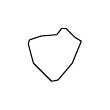
\begin{tikzpicture}
\draw (5.0789,3.9507) -- (4.9638,3.6711);
\draw (4.7664,4.0329) -- (4.5691,4.0164);
\draw (4.7007,3.4408) -- (4.4704,3.6711);
\draw (4.4046,3.9178) -- (4.4704,3.6711);
\draw (4.7829,3.4572) -- (4.7007,3.4408);
\draw (4.8816,4.1151) -- (4.9967,4.0000);
\draw (4.4211,3.9671) -- (4.5691,4.0164);
\draw (4.8322,4.1151) -- (4.8816,4.1151);
\draw (4.8322,4.1151) -- (4.7664,4.0329);
\draw (4.9967,4.0000) -- (5.0789,3.9507);
\draw (4.4211,3.9671) -- (4.4046,3.9178);
\draw (4.9638,3.6711) -- (4.7829,3.4572);
\fill (4.4211,3.9671) circle;
\fill (4.5691,4.0164) circle;
\fill (4.9967,4.0000) circle;
\fill (5.0789,3.9507) circle;
\fill (4.9638,3.6711) circle;
\fill (4.7829,3.4572) circle;
\fill (4.7007,3.4408) circle;
\fill (4.4704,3.6711) circle;
\fill (4.4046,3.9178) circle;
\fill (4.8322,4.1151) circle;
\fill (4.8816,4.1151) circle;
\fill (4.7664,4.0329) circle;
\end{tikzpicture}

\caption{$\textsc{minWeight} = -0.2$}
\label{fig:exp:multiple_weight:-0.2}
\end{subfigure}%
\begin{subfigure}{.25\linewidth}
\centering
%% Include the picture as follows: \
% \begingroup
% \tikzset{every picture/.style={scale=1,radius=0.05,line width=0.4}}%
% \input{tikz/[filename].tex}%
% \endgroup
%
%% Want to add a label? Use node[<position>]{label},
%% where <position> is one of: below / above / left / right
% \fill (0,0) circle node[below]{$p_1$};
%% Want to give the point a different color?
% \fill[red] (0,0) circle;
%
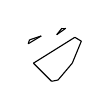
\begin{tikzpicture}
\draw (4.7829,3.4572) -- (4.7007,3.4408);
\draw (4.9967,4.0000) -- (4.4704,3.6711);
\draw (4.4211,3.9671) -- (4.5691,4.0164);
\draw (4.9638,3.6711) -- (4.7829,3.4572);
\draw (4.5691,4.0164) -- (4.4046,3.9178);
\draw (4.7007,3.4408) -- (4.4704,3.6711);
\draw (4.8816,4.1151) -- (4.7664,4.0329);
\draw (4.8322,4.1151) -- (4.8816,4.1151);
\draw (4.4211,3.9671) -- (4.4046,3.9178);
\draw (5.0789,3.9507) -- (4.9638,3.6711);
\draw (4.8322,4.1151) -- (4.7664,4.0329);
\draw (4.9967,4.0000) -- (5.0789,3.9507);
\fill (4.4211,3.9671) circle;
\fill (4.5691,4.0164) circle;
\fill (4.9967,4.0000) circle;
\fill (5.0789,3.9507) circle;
\fill (4.9638,3.6711) circle;
\fill (4.7829,3.4572) circle;
\fill (4.7007,3.4408) circle;
\fill (4.4704,3.6711) circle;
\fill (4.4046,3.9178) circle;
\fill (4.8322,4.1151) circle;
\fill (4.8816,4.1151) circle;
\fill (4.7664,4.0329) circle;
\end{tikzpicture}

\caption{$\textsc{minWeight} = 2$}
\label{fig:exp:multiple_weight:1}
\end{subfigure}
\caption{Varying $\textsc{minWeight}$}
\label{fig:exp:multiple_weight}
\end{figure}
\endgroup

Figure \ref{fig:exp:multiple_bar} shows an initial solution that consists of four curves.
With $\textsc{ClosenessFactor} = 1000$, the proximity of points is effectively not taken into account. The result of this becomes apparent in figure \ref{fig:exp:multiple_bar:bad}: the final curve looks like a bar with a dent. After setting the parameter to $5$, the dent disappears.

\begingroup
\tikzset{every picture/.style={scale=1,radius=0.05,line width=0.4,rotate=90}}%
\begin{figure}[ht!]
\centering
\begin{subfigure}{.25\linewidth}
\centering
%% Include the picture as follows: \
% \begingroup
% \tikzset{every picture/.style={scale=1,radius=0.05,line width=0.4}}%
% \input{tikz/[filename].tex}%
% \endgroup
%
%% Want to add a label? Use node[<position>]{label},
%% where <position> is one of: below / above / left / right
% \fill (0,0) circle node[below]{$p_1$};
%% Want to give the point a different color?
% \fill[red] (0,0) circle;
%
\begin{tikzpicture}
\fill (7.9243,6.3618) circle;
\fill (7.9572,5.0954) circle;
\fill (7.7928,4.0592) circle;
\fill (7.6941,3.5329) circle;
\fill (8.6974,6.7730) circle;
\fill (8.5658,6.0822) circle;
\fill (8.4836,5.3257) circle;
\fill (8.5164,4.7664) circle;
\fill (8.5987,3.9770) circle;
\fill (8.5987,3.2697) circle;
\end{tikzpicture}

\caption{Input}
\label{fig:exp:multiple_bar:input}
\end{subfigure}%
\begin{subfigure}{.25\linewidth}
\centering
%% Include the picture as follows: \
% \begingroup
% \tikzset{every picture/.style={scale=1,radius=0.05,line width=0.4}}%
% \input{tikz/[filename].tex}%
% \endgroup
%
%% Want to add a label? Use node[<position>]{label},
%% where <position> is one of: below / above / left / right
% \fill (0,0) circle node[below]{$p_1$};
%% Want to give the point a different color?
% \fill[red] (0,0) circle;
%
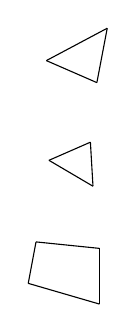
\begin{tikzpicture}
\draw (7.9572,5.0954) -- (8.5164,4.7664);
\draw (7.9572,5.0954) -- (8.4836,5.3257);
\draw (7.6941,3.5329) -- (8.5987,3.2697);
\draw (8.5987,3.9770) -- (8.5987,3.2697);
\draw (7.7928,4.0592) -- (8.5987,3.9770);
\draw (7.7928,4.0592) -- (7.6941,3.5329);
\draw (8.6974,6.7730) -- (8.5658,6.0822);
\draw (8.4836,5.3257) -- (8.5164,4.7664);
\draw (7.9243,6.3618) -- (8.6974,6.7730);
\draw (7.9243,6.3618) -- (8.5658,6.0822);
\fill (7.9243,6.3618) circle;
\fill (7.9572,5.0954) circle;
\fill (7.7928,4.0592) circle;
\fill (7.6941,3.5329) circle;
\fill (8.6974,6.7730) circle;
\fill (8.5658,6.0822) circle;
\fill (8.4836,5.3257) circle;
\fill (8.5164,4.7664) circle;
\fill (8.5987,3.9770) circle;
\fill (8.5987,3.2697) circle;
\end{tikzpicture}

\caption{Initial solution}
\label{fig:exp:multiple_bar:initial}
\end{subfigure}%
\begin{subfigure}{.25\linewidth}
\centering
%% Include the picture as follows: \
% \begingroup
% \tikzset{every picture/.style={scale=1,radius=0.05,line width=0.4}}%
% \input{tikz/[filename].tex}%
% \endgroup
%
%% Want to add a label? Use node[<position>]{label},
%% where <position> is one of: below / above / left / right
% \fill (0,0) circle node[below]{$p_1$};
%% Want to give the point a different color?
% \fill[red] (0,0) circle;
%
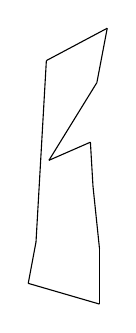
\begin{tikzpicture}
\draw (7.9572,5.0954) -- (8.4836,5.3257);
\draw (7.6941,3.5329) -- (8.5987,3.2697);
\draw (8.5987,3.9770) -- (8.5987,3.2697);
\draw (8.5164,4.7664) -- (8.5987,3.9770);
\draw (8.5658,6.0822) -- (7.9572,5.0954);
\draw (7.7928,4.0592) -- (7.6941,3.5329);
\draw (7.9243,6.3618) -- (7.7928,4.0592);
\draw (8.4836,5.3257) -- (8.5164,4.7664);
\draw (8.6974,6.7730) -- (8.5658,6.0822);
\draw (7.9243,6.3618) -- (8.6974,6.7730);
\fill (7.9243,6.3618) circle;
\fill (7.9572,5.0954) circle;
\fill (7.7928,4.0592) circle;
\fill (7.6941,3.5329) circle;
\fill (8.6974,6.7730) circle;
\fill (8.5658,6.0822) circle;
\fill (8.4836,5.3257) circle;
\fill (8.5164,4.7664) circle;
\fill (8.5987,3.9770) circle;
\fill (8.5987,3.2697) circle;
\end{tikzpicture}

\caption{$1000$}
\label{fig:exp:multiple_bar:bad}
\end{subfigure}%
\begin{subfigure}{.25\linewidth}
\centering
%% Include the picture as follows: \
% \begingroup
% \tikzset{every picture/.style={scale=1,radius=0.05,line width=0.4}}%
% \input{tikz/[filename].tex}%
% \endgroup
%
%% Want to add a label? Use node[<position>]{label},
%% where <position> is one of: below / above / left / right
% \fill (0,0) circle node[below]{$p_1$};
%% Want to give the point a different color?
% \fill[red] (0,0) circle;
%
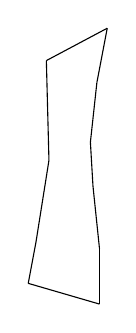
\begin{tikzpicture}
\draw (7.6941,3.5329) -- (8.5987,3.2697);
\draw (8.5987,3.9770) -- (8.5987,3.2697);
\draw (8.5164,4.7664) -- (8.5987,3.9770);
\draw (7.9572,5.0954) -- (7.7928,4.0592);
\draw (7.9572,5.0954) -- (7.9243,6.3618);
\draw (8.4836,5.3257) -- (8.5658,6.0822);
\draw (7.7928,4.0592) -- (7.6941,3.5329);
\draw (8.6974,6.7730) -- (8.5658,6.0822);
\draw (8.4836,5.3257) -- (8.5164,4.7664);
\draw (7.9243,6.3618) -- (8.6974,6.7730);
\fill (7.9243,6.3618) circle;
\fill (7.9572,5.0954) circle;
\fill (7.7928,4.0592) circle;
\fill (7.6941,3.5329) circle;
\fill (8.6974,6.7730) circle;
\fill (8.5658,6.0822) circle;
\fill (8.4836,5.3257) circle;
\fill (8.5164,4.7664) circle;
\fill (8.5987,3.9770) circle;
\fill (8.5987,3.2697) circle;
\end{tikzpicture}

\caption{factor $5$}
\label{fig:exp:multiple_bar:good}
\end{subfigure}
\caption{Initial solution and output for varying $\textsc{ClosenessFactor}$}
\label{fig:exp:multiple_bar}
\end{figure}
\endgroup

The previous evaluations shows that the initial solution is often close to the desired result, especially for dense curves. Many errors related to sparseness of a curve are correctly identified and resolved. The algorithm fails to provide the correct output when it mistakenly detects a group of points as one curve. This problem shows up for parallel lines that are close to each other, and also for dense curves with an uneven point distribution.

\subsubsection{Network reconstruction}
For this experimental evaluation the algorithm was run on several different input sets and with different parameters. The parameter $d_{max}$ is equal to the average length of the segments of the $EMST$ multiplied by a constant. Experimental evaluation showed that this constant should be around $2.5$. The parameter $\alpha_{straight}$ is set to $170\degree$ and $\alpha_{min}$ is set to $165\degree$. In the experimental evaluation below it shown that these values give the best result overall.
\begin{figure}[h]
\centering
  \begin{subfigure}{.4\linewidth}
  \centering
  \graphicspath{ {images/}}
  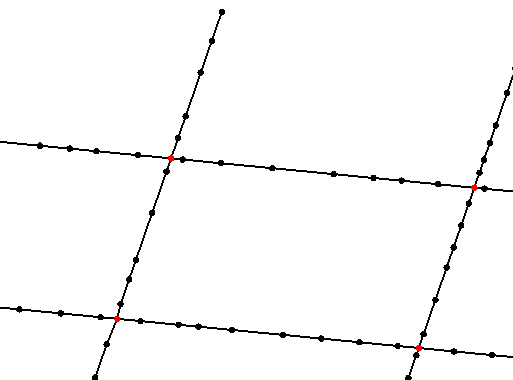
\includegraphics[width=\linewidth]{given167_170}
  \caption{$\alpha_{min}=165$ and $\alpha_{straight}=170$. }
  \label{givena}
  \end{subfigure}
    \begin{subfigure}{0.4\linewidth}
  \centering
  \graphicspath{ {images/}}
  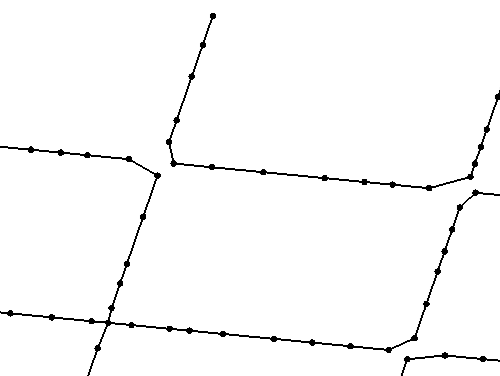
\includegraphics[width=\linewidth]{given90_90}
  \caption{$\alpha_{min}=130$ and $\alpha_{straight}=170$.}
  \label{givenb}
  \end{subfigure}
  \caption{}
  \label{given}
\end{figure}

Figure \ref{given} shows the output of the algorithm of a test case with straight roads and junctions. \ref{givena} shows the output with $\alpha_{min}=165$ and $\alpha_{straight}=170$ and \ref{givenb} shows the output with $\alpha_{min}=90$ and $\alpha_{straight}=170$. A crucial step in the algorithm is to identify straight road segments. A straight road segment consists of three points that make up two consecutive segments of which the middle point has degree 2. For a perfectly straight road the angle between these two segment is $180\degree$. But in our input straight roads could have a slight bend, therefore we set a margin of $10\degree$ by setting $\alpha_{straight}=170$. It is clear that figure \ref{givena} gives a better solution than figure \ref{givenb}. In figure \ref{givenb} any angle greater than $130\degree$ between two consecutive road segment is allowed. In figure \ref{givena} only angles greater than $165\degree$ between two consecutive road segments are allowed. Therefore the segments with a smaller angle, that were not removed in figure \ref{givenb}, are removed and connected to a point that gives an angle smaller than $165\degree$.

\begin{figure}[h]
\centering
  \begin{subfigure}{0.4\linewidth}
  \centering
  \graphicspath{ {images/}}
  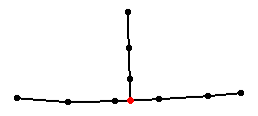
\includegraphics[width=\linewidth]{test1165_170}
  \caption{$\alpha_{min}=165$ and $\alpha_{straight}=170$.}
  \label{tjunctiona}
  \end{subfigure}
    \begin{subfigure}{0.4\linewidth}
  \centering
  \graphicspath{ {images/}}
  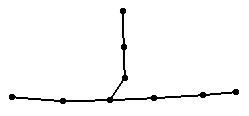
\includegraphics[width=\linewidth]{test1140_170}
  \caption{$\alpha_{min}=160$ and $\alpha_{straight}=170$.}
  \label{tjunctionb}
  \end{subfigure}
  \caption{}
\label{tjunction}
\end{figure}

Figure \ref{tjunction} shows a specific situation of a t-junction. With $\alpha_{min}=160$ the divergent segment in figure \ref{tjunctionb} is not removed. But with $\alpha_{min}=165$ the segment is removed, see figure \ref{tjunctiona} and a segment is added that connects to the new red point. Thus the angle, between the divergent segment and the segment above it, is greater than $160\degree$ and smaller than $165\degree$. It is arguable that the divergent segment should be removed because a real road could have a slight bend towards a t-junction. By observing several cases $\alpha_{min}=165$ seems close to the optimal setting.

\begin{figure}[h]
\centering
  \begin{subfigure}{0.4\linewidth}
  \centering
  \graphicspath{ {images/}}
  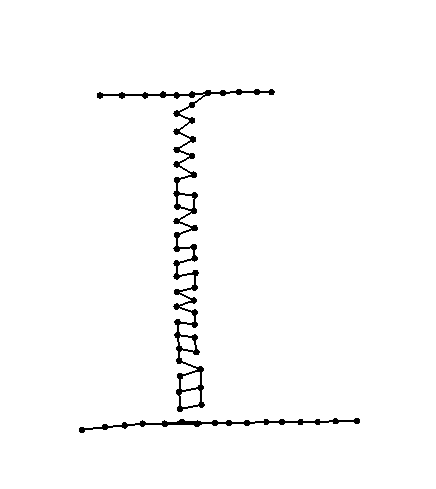
\includegraphics[width=\linewidth]{parallel165_165}
  \caption{$\alpha_{min}=165$ and $\alpha_{straight}=170$.}
  \label{parallel}
  \end{subfigure}
    \begin{subfigure}{0.4\linewidth}
  \centering
  \graphicspath{ {images/}}
  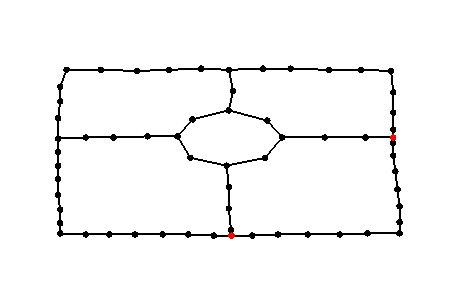
\includegraphics[width=\linewidth]{roundabout167_170}
  \caption{$\alpha_{min}=165$ and $\alpha_{straight}=170$.}
  \label{roundabout}
  \end{subfigure}
  \caption{}
  \label{testcases}
\end{figure}

In figure \ref{testcases} two different cases are shown. In the first case, figure \ref{parallel}, it is clear that the algorithm doesn't give an optimal solution. The algorithm's initial step creates a $EMST$, thus connecting the points with minimum total distance. This doesn't work well for parallel roads if the distance between the points that belong the same road is greater than the distance between points from both roads. The $EMST$ then connects the points that are closest to each other and thus connects points that should be in different roads. The next step of the algorithm looks for straight road segments and tries to improve the road network from there. However, as figure \ref{parallel} shows, the two parallel roads do not contain a straight road consisting of two straight segments of which the middle point has degree 2. Therefore the algorithm is not able to improve on this solution.

Figure \ref{roundabout} shows a test case with a roundabout and several t-junctions. The algorithm seems the give the optimal solution for this particular input. The roundabout is created by the first two steps of the algorithm. First the $EMST$ is created which nearly completes the roundabout and then point with degree 1 are connected to a nearby point, which works very well in this case. Also the t-junctions are connected in the right way with the given parameters.

\begin{figure}[h]
  \centering
  \graphicspath{ {images/}}
  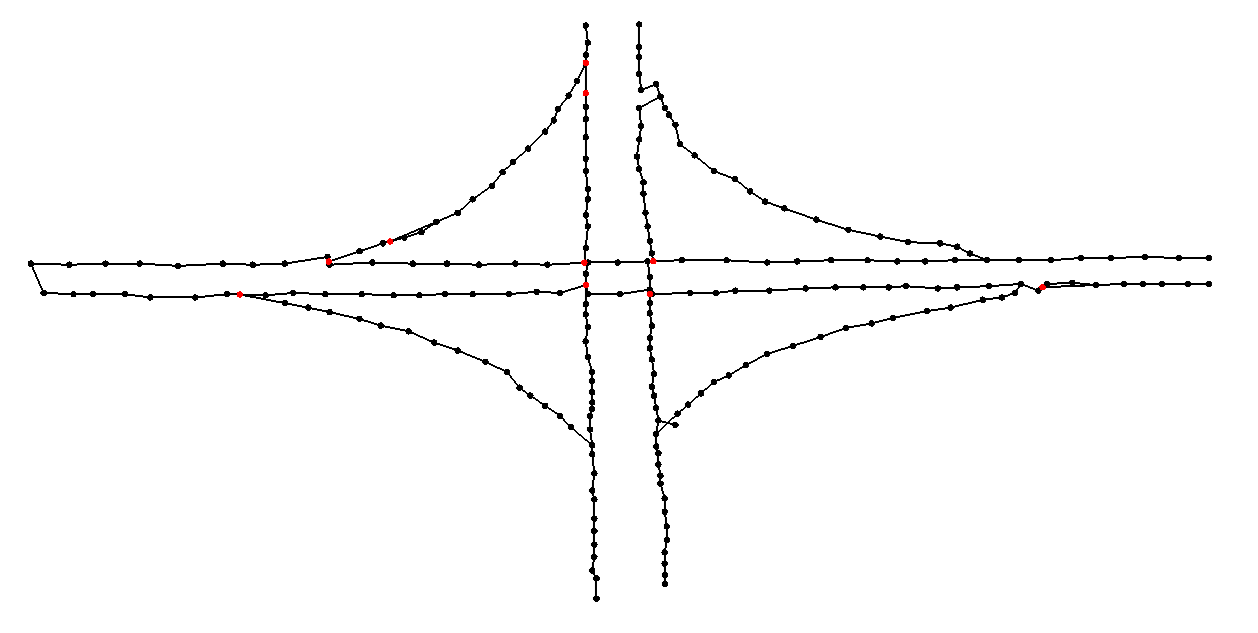
\includegraphics[width=\linewidth, height=150pt]{knooppunt167_170}
  \caption{$\alpha_{min}=165$ and $\alpha_{straight}=170$.}
  \label{knooppunt}
\end{figure}

Figure \ref{knooppunt} shows an input case with parallel roads for which the algorithm gives a fairly good solution. Because there is some space between the two parallel roads the $EMST$ doesn't connect two points that don't belong to the same road.

%TODO Move to Concluding remarks?
The experimental evaluation showed that the algorithm doesn't always give the optimal solution, but in most cases it comes close and sometimes it does give the optimal solution. The algorithm works very well for junctions and t-junctions, if the parameters are set correctly, which can be seen clearly in figure \ref{givena} and figure \ref{tjunctiona}. For parallel roads it doesn't always give an optimal solution, especially when the two roads are close to each other. This can be seen in figure \ref{parallel}. In cases where there is more distance between two parallel roads the algorithm works fairly well, as can be seen in figure \ref{knooppunt}. In future work the output for cases with parallel roads could be improved.


\section{Concluding remarks}
%TODO Multiple: future=Repeat step 1 with remaining points



\subsection{Future Work}
\bibliographystyle{plain}

\begin{thebibliography}{50}

\bibitem{crust}

Amenta, Nina, Marshall Bern, and Manolis Kamvysselis.
"A new Voronoi-based surface reconstruction algorithm."
\textit{Proceedings of the 25th annual conference on Computer graphics and interactive techniques}, 1998.

\bibitem{kruskal}
J.B. Kruskal.
On the shortest spanning subtree of a graph and the traveling salesman problem.
In \emph{Proceedings of the American Mathematical Society},7: 48-50, 1956.

\bibitem{chen}
D. Chen, L.J. Guibas, J. Hershberger, J. Sun.
Road Network Reconstruction for Organizing Paths.
In \emph{Proceedings  of  21st  ACM-SIAM  Symposium  on  Discrete  Algorithms}, 10: 1309-1320, 2010.

\bibitem{discur}
Zeng, Yong, et al. "A distance-based parameter free algorithm for curve reconstruction." \textit{Computer-Aided Design} 40.2: 210-222, 2008 .

\bibitem{gathan}
Dey, Tamal K., and Rephael Wenger. "Reconstruction curves with sharp corners." \textit{Proceedings of the sixteenth annual symposium on Computational geometry.} ACM, 2000.

\bibitem{convex}
Graham, R. L. "An efficient algorith for determining the convex hull of a finite planar set". \textit{Information processing letters}, 1(4), 132-133, 1972.

\bibitem{p-scnsg-57}
R. C. Prim.
Shortest connection networks and some generalizations.
In \emph{Bell System Technical Journal)}, 36: (1957), pp. 1389–1401

\bibitem{clrs-ia-09}
T.H. Cormen, C.E. Leiserson, R.L. Rivest, C. Stein.
\emph{Introduction to Algorithms} (3th edition).
The MIT Press, 2009.

\bibitem{cghs-rnrop-20}
D. Chen, L.J. Guibas, J. Hershberger, J. Sun.
Road Network Reconstruction for Organizing Paths.
In \emph{Proceedings of 21st ACM-SIAM Symposium on Discrete Algorithms}, 10: 1309-1320, 2010.

\end{thebibliography}







\end{document}
